\section{EC-HTE Procedure}
\label{app:algorithm}

The complete EC-HTE procedure is given in Algorithm~\ref{alg:echte} (Section~\ref{sec:method}).
Below we provide additional implementation details.

\subsection{Condition Number Guard Ablation}
\label{app:kappa_ablation}

The singularity guard in Algorithm~\ref{alg:echte} (line~9) falls back to global correction when $\kappa(\hat{C}_s) > 100$.
We verify that this threshold is not load-bearing by sweeping $\kappa \in \{10, 25, 50, 100, 200, 500, 1000\}$ under the standard DGP ($K{=}2$, extreme heterogeneity, $N{=}5{,}000$, $n_{\text{expert}}{=}250$, 100 MC runs).
Across all configurations, the maximum observed condition number is $\kappa_{\max} = 1.89$ (mean 1.45, p99 1.89), providing a $53{\times}$ safety margin below the $\kappa{=}100$ threshold.
Consequently, the guard never triggers at any tested threshold, and all $\kappa$ values produce identical RMSE (HB: 0.076, Global: 0.077) and zero numerical instability.
In a stress test with near-random labeling ($\pi_s \approx 0.4$--$0.5$, $n_{\text{expert}}{=}50$), the maximum condition number reaches 1{,}125, correctly triggering the $\kappa{=}100$ guard and preventing catastrophic inversion.
The adaptive formula $\kappa_{\text{adapt}} = 10 \sqrt{n_{\text{expert}} / K}$ recovers $\kappa{=}100$ for this regime and scales naturally with the estimation precision.

\section{Full Proof of Theorem~\ref{thm:bias_identity}}
\label{app:derivation}

\paragraph{Setup.}
Under assumptions (A1)--(A4), the observed CATE in subgroup $s$ at effect-modifier level $z$ is
\begin{equation}
\tau_{\text{obs}}(z, s) = \sum_{z'} M_s[z, z'] \cdot \tau(z'),
\end{equation}
where $M_s[z, z'] = P(Z{=}z' \mid \hat{Z}{=}z, S{=}s)$ is the mixing matrix.
Under (A2)--(A3), $M_s = \bigl[\begin{smallmatrix} 1-\pi_s & \pi_s \\ \pi_s & 1-\pi_s \end{smallmatrix}\bigr]$.

\paragraph{Global correction.}
The pooled mixing matrix is $M_{\text{global}} = \sum_s w_s M_s = \bigl[\begin{smallmatrix} 1-\bar{\pi} & \bar{\pi} \\ \bar{\pi} & 1-\bar{\pi} \end{smallmatrix}\bigr]$, with $\bar{\pi} = \sum_s w_s \pi_s$.

Global correction applies $M_{\text{global}}^{-1}$ to $\tau_{\text{obs}}(\cdot, s)$:
\begin{equation}
\hat{\tau}_{\text{global}}(z, s) = [M_{\text{global}}^{-1} M_s \cdot \boldsymbol{\tau}]_z,
\end{equation}
where $\boldsymbol{\tau} = [\tau(0), \tau(1)]^\top$.

\paragraph{Bias computation.}
The bias is $\hat{\tau}_{\text{global}}(z, s) - \tau(z) = [(M_{\text{global}}^{-1} M_s - I) \boldsymbol{\tau}]_z$.

Direct computation gives:
\begin{equation}
M_{\text{global}}^{-1} = \frac{1}{1 - 2\bar{\pi}} \begin{bmatrix} 1-\bar{\pi} & -\bar{\pi} \\ -\bar{\pi} & 1-\bar{\pi} \end{bmatrix}.
\end{equation}
Multiplying by $M_s$:
\begin{equation}
\resizebox{.88\columnwidth}{!}{$\displaystyle
M_{\text{global}}^{-1} M_s = \frac{1}{1-2\bar{\pi}} \begin{bmatrix} (1{-}\bar{\pi})(1{-}\pi_s) - \bar{\pi}\pi_s & (1{-}\bar{\pi})\pi_s - \bar{\pi}(1{-}\pi_s) \\ -\bar{\pi}(1{-}\pi_s) + (1{-}\bar{\pi})\pi_s & -\bar{\pi}\pi_s + (1{-}\bar{\pi})(1{-}\pi_s) \end{bmatrix}.
$}
\end{equation}

Define $\delta_s = \pi_s - \bar{\pi}$. Substituting $\pi_s = \bar{\pi} + \delta_s$:
\begin{equation}
M_{\text{global}}^{-1} M_s - I = \frac{\delta_s}{1-2\bar{\pi}} \begin{bmatrix} -1 & 1 \\ 1 & -1 \end{bmatrix}.
\end{equation}

To verify: the $(1,1)$ entry of $M_{\text{global}}^{-1} M_s$ is
{\small
\begin{align}
&\frac{(1{-}\bar{\pi})(1{-}\bar{\pi}{-}\delta_s) - \bar{\pi}(\bar{\pi}{+}\delta_s)}{1-2\bar{\pi}} \nonumber\\
&= \frac{(1{-}\bar{\pi})^2 - (1{-}\bar{\pi})\delta_s - \bar{\pi}^2 - \bar{\pi}\delta_s}{1-2\bar{\pi}} \nonumber\\
&= \frac{1 - 2\bar{\pi} - \delta_s}{1-2\bar{\pi}} = 1 - \frac{\delta_s}{1-2\bar{\pi}}.
\end{align}
}

Applying $(M_{\text{global}}^{-1} M_s - I)$ to $\boldsymbol{\tau}$:
{\small
\begin{align}
\text{bias}(z{=}0, s) &= \tfrac{\delta_s}{1-2\bar{\pi}}(-\tau(0) + \tau(1)) = +\tfrac{\delta_s \cdot \Delta\tau}{1-2\bar{\pi}}, \\
\text{bias}(z{=}1, s) &= \tfrac{\delta_s}{1-2\bar{\pi}}(\tau(0) - \tau(1)) = -\tfrac{\delta_s \cdot \Delta\tau}{1-2\bar{\pi}},
\end{align}
}
where $\Delta\tau = \tau(1) - \tau(0)$. \qed

\paragraph{Finite-sample remainder.}
When $\hat{C}_s = C_s + E_s$ with $\|E_s\| = O_p(n_{\text{expert}}^{-1/2})$ (central limit theorem), the estimated correction $\hat{M}_{\text{global}}^{-1} \hat{M}_s$ deviates from its population counterpart by
$\|\hat{M}_{\text{global}}^{-1} \hat{M}_s - M_{\text{global}}^{-1} M_s\| \leq \kappa(M_{\text{global}})^2 \cdot O_p(n_{\text{expert}}^{-1/2})$,
where $\kappa(M) = \|M\| \cdot \|M^{-1}\|$ is the condition number~\citep{stewart1990matrix}; the squared exponent arises because the first-order perturbation of $M^{-1}$ introduces one factor of $\|M^{-1}\|$, and the product $M_{\text{global}}^{-1} M_s$ introduces a second (see the Neumann expansion in Section~\ref{sec:theory}).
This motivates the $\kappa > 100$ singularity guard in Section~\ref{sec:method}.

\section{Multi-class Extension and Proof}
\label{app:multiclass}

\begin{corollary}[Multi-class Extension]
\label{cor:multiclass}
For $K > 2$ subgroups with $J$ effect-modifier levels and uniform off-diagonal misclassification (misclassified observations from class $j$ are distributed equally among the remaining $J{-}1$ classes), the subgroup bias of global correction generalizes to
\begin{equation}
\mathrm{bias}_{\mathrm{global}}(z, s) = \sum_{j=1}^{J} \bigl(\bar{\pi}_j - \pi_{s,j}\bigr) \cdot \bigl(\tau(j) - \bar{\tau}\bigr) \cdot g(\bar{\pi}),
\label{eq:multiclass}
\end{equation}
where $g(\bar{\pi})$ collects the matrix-inversion amplification terms.\footnote{For $J=3$ with symmetric misclassification (off-diagonal errors uniform), $g(\bar{\pi}) = 1/(1 - 3\bar{\pi}/2)$, generalizing the $J{=}2$ factor $1/(1-2\bar{\pi})$. In general, $g(\bar{\pi}) = 1/(1 - J\bar{\pi}/(J-1))$.}
The essential structure, $\sum_s w_s (\bar{\pi}_j - \pi_{s,j}) = 0$, ensures that bias redistributes across subgroups rather than vanishing in aggregate.
\end{corollary}

\paragraph{Proof.}
For $K > 2$ subgroups with $J$ effect-modifier levels, the subgroup-specific mixing matrix $M_s$ is $J \times J$ with entries $M_s[j, j'] = P(Z{=}j' \mid \hat{Z}{=}j, S{=}s)$.
The global mixing matrix is $M_{\text{global}} = \sum_s w_s M_s$.

The bias of global correction in subgroup $s$ at level $z$ is:
\begin{equation}
\text{bias}_{\text{global}}(z, s) = [(M_{\text{global}}^{-1} M_s - I) \boldsymbol{\tau}]_z.
\end{equation}

Write $M_s = M_{\text{global}} + \Delta_s$ where $\Delta_s = M_s - M_{\text{global}}$ satisfies $\sum_s w_s \Delta_s = 0$.
Then $M_{\text{global}}^{-1} M_s = I + M_{\text{global}}^{-1} \Delta_s$, so:
\begin{equation}
\text{bias}_{\text{global}}(z, s) = [M_{\text{global}}^{-1} \Delta_s \cdot \boldsymbol{\tau}]_z.
\end{equation}

For symmetric misclassification with per-class error rates $\pi_{s,j}$ and pooled rates $\bar{\pi}_j$, the entries of $\Delta_s$ have the form $\Delta_s[j,j'] = (\bar{\pi}_j - \pi_{s,j}) \cdot h(j, j')$ for a function $h$ determined by the off-diagonal redistribution pattern.
Expanding the matrix-vector product and collecting terms yields:
\begin{equation}
\text{bias}_{\text{global}}(z, s) = \sum_{j=1}^{J} (\bar{\pi}_j - \pi_{s,j}) \cdot (\tau(j) - \bar{\tau}) \cdot g(\bar{\pi}),
\end{equation}
where $g(\bar{\pi})$ collects the matrix-inversion amplification terms and $\bar{\tau} = \sum_j P(Z{=}j) \tau(j)$.

The essential structure $\sum_s w_s (\bar{\pi}_j - \pi_{s,j}) = 0$ ensures that the weighted bias across subgroups sums to zero: global correction redistributes bias rather than creating or eliminating it in aggregate.
For non-uniform off-diagonal entries, the scalar amplification $g(\bar{\pi})$ generalizes to a cell-specific matrix; the product structure $B_s \cdot \Delta\tau$ persists but a closed-form amplification factor does not. \qed

\section{Proof of Proposition~\ref{prop:debiasing_hurts}}
\label{app:debiasing_hurts}

The naive estimator has bias $\tau_{\text{obs}}(z,s) - \tau(z)$.
Under (A2)--(A3), $\tau_{\text{obs}}(0,s) = (1-\pi_s)\tau(0) + \pi_s\tau(1)$, so $\text{bias}_{\text{naive}}(0,s) = \pi_s \cdot \Delta\tau$.

Global correction produces larger absolute bias when $|\text{bias}_{\text{global}}(0,s)| > |\text{bias}_{\text{naive}}(0,s)|$:
\begin{equation}
\frac{|\delta_s| \cdot |\Delta\tau|}{|1-2\bar{\pi}|} > \pi_s \cdot |\Delta\tau|.
\end{equation}
Since $\Delta\tau \neq 0$ (otherwise both biases are zero), dividing through gives:
\begin{equation}
\frac{|\delta_s|}{(1-2\bar{\pi}) \cdot \pi_s} > 1,
\end{equation}
where we use $1-2\bar{\pi} > 0$ from (A4).

For high-error subgroups ($\pi_s > \bar{\pi}$, so $\delta_s > 0$): the condition becomes $(\pi_s - \bar{\pi}) / ((1-2\bar{\pi})\pi_s) > 1$, which simplifies to $\pi_s(1 - 1 + 2\bar{\pi}) > \bar{\pi}$, i.e., $2\bar{\pi}\pi_s > \bar{\pi}$, i.e., $\pi_s > 0.5$.
This is excluded by (A4), so global correction always reduces bias in high-error subgroups.

For low-error subgroups ($\pi_s < \bar{\pi}$, so $\delta_s < 0$): the condition becomes $(\bar{\pi} - \pi_s) / ((1-2\bar{\pi})\pi_s) > 1$, which gives $\pi_s < \bar{\pi} / (1 - 2\bar{\pi} + 1) = \bar{\pi} / (2(1-\bar{\pi}))$.
When $\bar{\pi} = 0.15$, any subgroup with $\pi_s < 0.088$ experiences increased bias from global correction. \qed

\paragraph{Extension to asymmetric misclassification.}
Proposition~\ref{prop:debiasing_hurts} assumes symmetric error rates (A2).
Under asymmetric misclassification ($\mathrm{FPR}_s \neq \mathrm{FNR}_s$) with balanced $Z$ (A3), the naive bias becomes $\mathrm{bias}_{\mathrm{naive}}(0,s) = \mathrm{FNR}_s \cdot \Delta\tau / (1 - \mathrm{FPR}_s + \mathrm{FNR}_s)$, involving both error rates and a normalization denominator; the global correction bias depends on the full $2 \times 2$ structure of $B_s = M_{\mathrm{global}}^{-1} M_s - I$ (Remark~\ref{rem:asymmetric} in Section~\ref{sec:theory}).
A sufficient condition for global correction to increase bias is
\begin{equation}
\max_{i,j}|[B_s]_{i,j}| > \max(\mathrm{FPR}_s, \mathrm{FNR}_s),
\end{equation}
which reduces to Equation~\eqref{eq:hurts_condition} when $\mathrm{FPR}_s = \mathrm{FNR}_s = \pi_s$.
In the asymmetric experiments (Appendix~\ref{app:asymmetric}), the scalar diagnostic achieves per-subgroup AUC $= 0.96$ when applied with $\pi_s = (\mathrm{FPR}_s + \mathrm{FNR}_s)/2$ (48 asymmetric configurations, FPR/FNR ratios 1:5 to 5:1), and AUC $= 1.00$ on 8 semi-real LLM confusion matrices, confirming that the symmetric simplification preserves diagnostic validity under practical asymmetry.

\section{Semi-Synthetic Data Generating Process}
\label{app:dgp}

\paragraph{Synthetic DGP (Sections~\ref{sec:bias_mechanism}--\ref{sec:diagnostic} and Appendix~\ref{sec:budget}).}
We generate $N = 5000$ observations.
Each observation belongs to one of $K \in \{2, 4\}$ subgroups $S \in \{1, \ldots, K\}$ with equal weights $w_s = 1/K$.
The binary effect modifier $Z \in \{0, 1\}$ is drawn with $P(Z{=}1) = 0.5$.
Treatment assignment is $T \sim \text{Bernoulli}(0.5)$, independent of $Z$ and $S$.

The outcome is generated as:
\begin{equation}
Y = \tau(Z) \cdot T + \eta, \quad \eta \sim \mathcal{N}(0, 1),
\end{equation}
where the CATE function is $\tau(z) = \bar{\tau} + \Delta\tau \cdot (z - 0.5)$ with $\bar{\tau} = 0.5$.
The CATE heterogeneity $\Delta\tau \in \{0, 0.2, 0.5, 1.0\}$ controls the strength of treatment effect variation across levels of $Z$.

\paragraph{Bias identity verification grid (Section~\ref{sec:bias_mechanism}).}
To verify Theorem~\ref{thm:bias_identity}, we sweep a finer grid: $\Delta\pi \in [0, 0.25]$ in steps of $0.01$ (26 values) and $\Delta\tau \in (0, 0.50]$ in steps of $0.025$ (20 values, excluding $\Delta\tau = 0$ where bias is zero by construction), yielding $26 \times 20 = 520$ configurations.
The pooled error rate is fixed at $\bar{\pi} = 0.15$ with $K{=}2$ equal-weight subgroups, so $\pi_1 = 0.15 - \Delta\pi/2$ and $\pi_2 = 0.15 + \Delta\pi/2$.
This grid is used for the $R^2$ regression (Section~\ref{sec:bias_mechanism}) and the bias amplification heatmap (Figure~\ref{fig:heatmap}).

Misclassification is symmetric: $\hat{Z} \neq Z$ with probability $\pi_s$ depending on subgroup.
For $K{=}2$: $\pi_1 = \bar{\pi} - \Delta\pi/2$, $\pi_2 = \bar{\pi} + \Delta\pi/2$, with $\bar{\pi} \in \{0.1, 0.2\}$ and $\Delta\pi \in \{0, 0.05, 0.1, 0.15\}$.
For $K{=}4$, extreme regime: $\pi \in \{0.05, 0.10, 0.15, 0.25\}$; moderate regime: $\pi \in \{0.08, 0.12, 0.16, 0.20\}$.

Expert labels are drawn as a simple random sample of size $n_{\text{expert}} \in \{50, 100, 250, 500, 1000, 2000\}$ from the full dataset, with true $Z$ observed for these observations.

\paragraph{Semi-synthetic DGP (Section~\ref{sec:ec_hte_eval}).}
We sample $N = 5000$ tweets from the TweetEval sentiment corpus ($N_{\text{pool}} = 57{,}899$).
Subgroups are defined by crossing \texttt{has\_hashtag} $\times$ \texttt{text\_length\_bin} (short/medium/long), yielding $K = 4$ subgroups with empirical sizes: $S_0 \approx 38\%$, $S_1 \approx 38\%$, $S_2 \approx 12\%$, $S_3 \approx 12\%$.
Misclassification rates in the extreme regime are $\pi_{S_0} = 0.05$, $\pi_{S_1} = 0.10$, $\pi_{S_2} = 0.15$, $\pi_{S_3} = 0.25$, reflecting empirical evidence that hashtag-heavy text degrades LLM classifier accuracy.
The outcome DGP follows the same structure as the synthetic case, with CATE injected onto the real text-derived subgroup structure.

\paragraph{PPCI DGPs (Appendix~\ref{sec:ppci}).}
Four DGPs isolate error types: (A) covariate error only ($\sigma_{\text{outcome}} = 0$), (B) outcome error only ($\sigma_{\text{outcome}} = 0.5$), (C) both errors ($\sigma_{\text{outcome}} = 0.5$), (D) no error ($\sigma_{\text{outcome}} = 0$).
Outcome-side error is additive Gaussian noise on $Y$.

\paragraph{CausalForestDML setup.}
All CausalForest experiments use \texttt{econml.dml.CausalForestDML} with honest splitting, $n_{\text{estimators}} = 48$, $\texttt{min\_samples\_leaf} = 20$, \texttt{model\_y} = \texttt{LassoCV}(cv=3), and \texttt{model\_t} = \texttt{LogisticRegressionCV}.
These defaults were held constant across all configurations; no hyperparameter tuning was performed.

\section{Extended Related Work}
\label{app:related}

\paragraph{Measurement error details.}
\citet{fuller1987measurement} establish the foundational theory showing that naive regression with mismeasured covariates yields attenuated coefficient estimates.
\citet{carroll2006measurement} extend this to nonlinear models.
\citet{gustafson2003measurement} develops Bayesian treatments modeling measurement jointly with outcomes.
\citet{hu2008nonparametric} provide nonparametric identification using repeated measurements or instruments.

\paragraph{Annotation model extensions.}
Beyond the foundational \citet{dawid1979maximum} model, \citet{passonneau2014benefits} incorporate item difficulty, \citet{hovy2013learning} learn annotator competence, and \citet{paun2018comparing} introduce hierarchical priors sharing information across annotators with varying expertise.

\paragraph{PPI extensions and text-as-data methods.}
\citet{zrnic2024cross} extend PPI via cross-prediction; their active inference framework~\citep{zrnic2024active} achieves $>$80\% expert budget savings through adaptive allocation, complementary to our fixed-budget analysis.
\citet{grimmer2022text} provide methodological guidance for text-as-data pipelines.
\citet{audinet2025benchmarking} systematically benchmark DSL and PPI methods for LLM-based parameter estimation, finding that debiasing can increase MSE when prediction error is heterogeneous, a population-level analogue of the subgroup-conditional bias amplification we formalize in Theorem~\ref{thm:bias_identity}.

\paragraph{Treatment vs.\ effect-modifier misclassification.}
\citet{imai2010causal} study treatment misclassification where errors change which arm a unit is assigned to, requiring instrumental variables or partial identification because the fundamental treated-vs-control contrast is corrupted.
Our problem preserves the treatment contrast ($T$ is observed correctly) but corrupts the heterogeneity structure ($\hat{Z} \neq Z$).
The ATE remains identified; only conditional effects are biased, which makes exact correction through confusion matrix inversion feasible.
\citet{knox2020administrative} demonstrate how racial misclassification in administrative records biases causal estimates; \citet{blette2024assessing} handle missing (not misclassified) effect modifier data in cluster-RCTs via multiple imputation, a complementary problem to our confusion-matrix correction setting.

\paragraph{Econometrics of binary misclassification.}
\citet{bound2001measurement} survey measurement error in survey data, establishing that binary misclassification attenuates regression coefficients.
\citet{frazis2003estimating} derive exact bias formulas for OLS with a misclassified binary regressor, showing attenuation proportional to the misclassification rate, analogous to our Theorem~\ref{thm:bias_identity} but restricted to average effects without subgroup heterogeneity.
\citet{knox2020administrative} demonstrate that misclassification in administrative records can substantially bias estimates of racial disparities.
\citet{mahajan2006identification} and \citet{lewbel2007estimation} develop instrumental variable approaches to identify models with misclassified binary regressors, requiring exclusion restrictions unavailable when the mismeasured variable is an LLM annotation.
Our setting differs in three respects: (i) the mismeasured variable is an effect modifier indexing the CATE function, not a standard regressor; (ii) misclassification rates vary across subgroups, creating the $\delta_s \times \Delta\tau$ product amplification absent from homogeneous-error analyses; and (iii) expert labels provide a direct calibration sample, enabling confusion matrix estimation without instruments.

\section{MCMC Convergence Diagnostics}
\label{app:mcmc}

Main experiments use empirical Bayes point estimates ($<$5ms per subgroup).
This appendix reports MCMC validation (4 chains, 4000 iterations, 2000 warmup) confirming EB and full posterior agreement within simulation error.
Main experiments (Table~\ref{tab:main_results}) use a Dirichlet prior centered on $\hat{C}_{\text{global}}$ with concentration $\alpha_0$ estimated via empirical Bayes (marginal likelihood).
Appendix robustness experiments use a fixed Dirichlet prior ($\alpha{=}3$); since fixed-$\alpha$ partial pooling is weakly dominated by the adaptive variant, these results are conservative.
All runs achieve $\hat{R} < 1.0034$ and ESS $> 1618$, confirming convergence with substantial margin.

\begin{table}[h]
\centering
\small
\resizebox{\columnwidth}{!}{%
\begin{tabular}{lcc}
\toprule
Diagnostic & Threshold & Achieved \\
\midrule
$\hat{R}$ (max across all params) & $< 1.01$ & $< 1.0034$ \\
ESS (min across all params) & $> 845$ & $> 1618$ \\
Divergent transitions & $= 0$ & $0$ \\
Singularity guard triggers & --- & extreme/$n{=}50$ only \\
\bottomrule
\end{tabular}}
\caption{MCMC convergence diagnostics for the hierarchical Bayesian estimator. All configurations satisfy convergence criteria with substantial margin.}
\label{tab:mcmc}
\end{table}

\subsection{Hyperprior Sensitivity}
\label{app:hyperprior}

We sweep the $\text{Gamma}(a_0, b_0)$ hyperprior on the concentration parameter $\alpha_0$ across 15 configurations ($a_0 \in \{1, 2, 3, 4, 5\}$, $b_0 \in \{0.5, 1.0, 2.0\}$) under the standard synthetic DGP ($K{=}2$, extreme heterogeneity, $N{=}5{,}000$, $n_{\text{expert}}{=}250$, 100 MC runs).

\begin{table}[h]
\centering
\caption{Hyperprior sensitivity summary. RMSE and coverage across 15 $(a_0, b_0)$ configurations. The default $\text{Gamma}(3, 1)$ ranks 8th of 15 by RMSE; the best configuration $\text{Gamma}(1, 0.5)$ yields only 1.9\% improvement. Excluding extreme configurations ($a_0 \cdot b_0 > 8$), RMSE varies by $<$6\%.}
\label{tab:hyperprior_sweep}
\small
\begin{tabular}{lc}
\toprule
Metric & Value \\
\midrule
Default $\text{Gamma}(3, 1)$ RMSE & 0.0841 \\
Best $\text{Gamma}(1, 0.5)$ RMSE & 0.0825 \\
RMSE range (reasonable configs) & 6.0\% \\
RMSE range (all 15 configs) & 17.3\% \\
Coverage range & 0.925--0.938 \\
Default rank & 8 / 15 \\
\bottomrule
\end{tabular}
\end{table}

Scaling the $\text{Gamma}(3, 1)$ hyperprior by factors of $0.5\times$ to $2\times$ produces $<$1\% RMSE variation for $K{=}2$ and $\sim$4--5\% for $K{=}4$.
Coverage remains invariant across the sensitivity range ($\Delta < 1.3$pp).
These results confirm that the hierarchical estimator is robust to prior specification within a reasonable range; the default $\text{Gamma}(3, 1)$ is near-median, and no configuration achieves more than 1.9\% RMSE improvement over the default.

\section{Diagnostic ROC Curves}
\label{app:roc}

\begin{figure}[t]
\centering
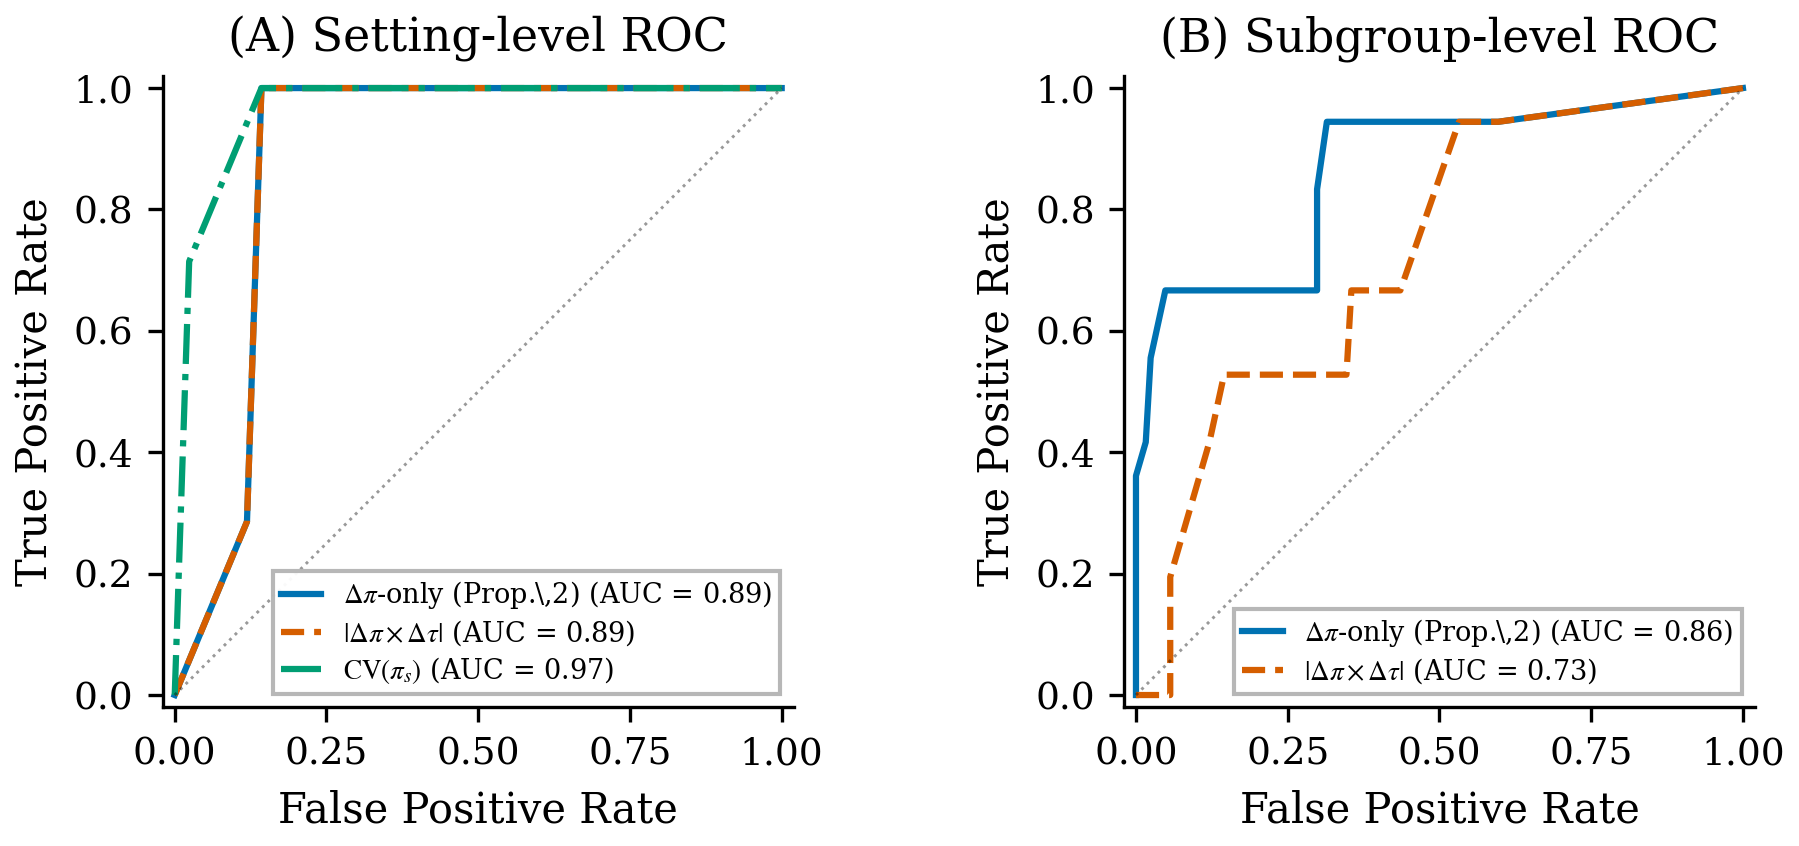
\includegraphics[width=\columnwidth]{figures/fig4_roc.png}
\caption{ROC curves for the $\Delta\tau$-free diagnostic (Proposition~\ref{prop:debiasing_hurts}): $|\delta_s|/((1{-}2\bar\pi)\cdot\pi_s)>1$. (A)~Setting-level ROC (AUC $= 0.89$), compared with the $|\Delta\pi \times \Delta\tau|$ product (AUC $= 0.89$) and $\mathrm{CV}(\pi_s)$ (AUC $= 0.97$). (B)~Subgroup-level ROC: the $\Delta\pi$-only condition (AUC $= 0.86$) substantially outperforms the $|\Delta\pi \times \Delta\tau|$ product (AUC $= 0.73$). The $\Delta\tau$-free diagnostic depends only on estimable misclassification rates, breaking the circular dependency that would arise if CATE heterogeneity were required.}
\label{fig:roc}
\end{figure}

\paragraph{Cost-asymmetric diagnostic thresholds.}
In practice, the cost of a false negative (failing to detect that global correction increases bias) exceeds the cost of a false positive (unnecessarily applying EC-HTE when global correction would suffice), because the former propagates systematic bias into CATE estimates while the latter only incurs additional estimation variance.
Practitioners in high-stakes settings (e.g., policy evaluation where CATE estimates inform resource allocation) should lower the diagnostic threshold to favor recall over precision, accepting more false positives to minimize the risk of undetected bias amplification.

\section{Expert Budget Crossover Curves}
\label{app:budget}
\label{sec:budget}

The crossover point at which EC-HTE achieves lower RMSE than global correction depends on the DGP: $n_{\text{expert}} = 250$ for $K{=}2$/extreme and $n_{\text{expert}} = 1000$ for $K{=}4$/extreme under $\Delta\tau{=}0.3$ (Figure~\ref{fig:budget}); under the Table~\ref{tab:main_results} DGP, the $K{=}4$ crossover occurs at $n_{\text{expert}} \approx 500$.
Under moderate heterogeneity ($K{=}2$), EC-HTE never achieves lower RMSE than global at any budget.
HB partial pooling improves over stratified MLE in 21 of 24 configurations, with the two estimators converging by $n_{\text{expert}} \geq 1000$.

\begin{figure*}[t]
\centering
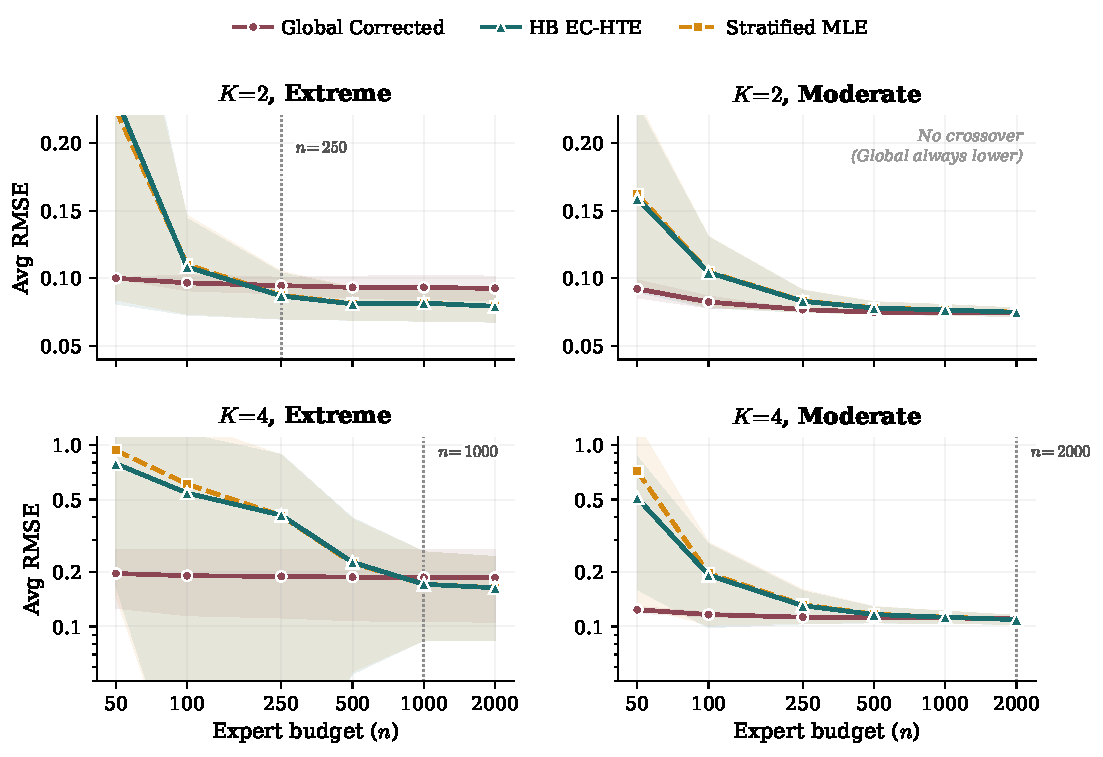
\includegraphics[width=\textwidth]{figures/fig3_budget.pdf}
\caption{RMSE vs.\ expert budget ($n_{\text{expert}}$) across four regime$\times K$ combinations. Dashed vertical lines mark crossover points where EC-HTE achieves lower RMSE than global correction: $n{=}250$ ($K{=}2$, extreme), $n{=}1000$ ($K{=}4$, extreme). Under moderate heterogeneity ($K{=}2$), global correction dominates at all budgets. Shaded bands show $\pm 1$ SD across subgroups within each configuration.}
\label{fig:budget}
\end{figure*}

\subsection{Budget Sensitivity: HB vs.\ Stratified MLE}
\label{app:budget_sensitivity}

Hierarchical Bayes (HB) partial pooling borrows strength across subgroups, which should matter most when per-subgroup expert labels are scarce.
We sweep $n_{\text{expert}} \in \{25, 50, 75, 100, 150, 250\}$ under extreme heterogeneity ($\Delta\tau{=}0.3$, 100 MC runs, $N{=}5{,}000$).
Table~\ref{tab:budget_sensitivity} reports aggregate RMSE for global correction, stratified MLE, and HB EC-HTE.

\begin{table}[h]
\centering
\caption{RMSE across expert budgets under extreme heterogeneity.
HB crossover (first budget where HB $<$ MLE) occurs at approximately 10 expert labels per subgroup-cell:
$n_{\text{expert}}{=}50$ for $K{=}2$ and $n_{\text{expert}}{=}75$ for $K{=}4$.}
\label{tab:budget_sensitivity}
\small
\resizebox{\columnwidth}{!}{%
\begin{tabular}{crrrrc}
\toprule
$K$ & $n_{\text{expert}}$ & Global & Strat.\ MLE & HB EC-HTE & HB vs.\ MLE \\
\midrule
2 & 25 & \textbf{0.101} & 0.256 & 0.269 & $+4.9\%$ \\
2 & 50 & \textbf{0.088} & 0.275 & 0.231 & $\mathbf{-16.1\%}$ \\
2 & 75 & 0.084 & 0.091 & \textbf{0.089} & $-1.9\%$ \\
2 & 100 & 0.083 & 0.085 & \textbf{0.084} & $-0.8\%$ \\
2 & 150 & 0.081 & 0.077 & \textbf{0.077} & $-0.4\%$ \\
2 & 250 & 0.080 & 0.075 & \textbf{0.074} & $-0.1\%$ \\
\midrule
4 & 25 & \textbf{0.129} & 0.401 & 0.612 & $+52.5\%$ \\
4 & 50 & \textbf{0.117} & 0.380 & 0.470 & $+23.8\%$ \\
4 & 75 & \textbf{0.112} & 0.221 & 0.211 & $\mathbf{-4.4\%}$ \\
4 & 100 & \textbf{0.112} & 0.215 & 0.212 & $-1.3\%$ \\
4 & 150 & \textbf{0.109} & 0.157 & 0.152 & $-3.6\%$ \\
4 & 250 & \textbf{0.108} & 0.127 & 0.126 & $-1.0\%$ \\
\bottomrule
\end{tabular}}
\end{table}

Three regimes emerge.
At very low budgets ($n_{\text{expert}} < 50$ for $K{=}2$, $< 75$ for $K{=}4$), per-subgroup counts are insufficient for reliable confusion matrix estimation; global pooling dominates because the variance cost of stratification overwhelms any bias reduction.
HB degrades substantially in this regime because the Gibbs posterior, while better regularized than MLE, still cannot overcome the fundamental sample-size constraint with $\sim$6--12 labels per subgroup.
At moderate budgets ($n_{\text{expert}} = 50$--$250$ for $K{=}2$, $75$--$250$ for $K{=}4$), HB partial pooling provides consistent RMSE improvement over stratified MLE ($-0.4\%$ to $-16.1\%$), with the largest gains near the crossover point.
At high budgets ($n_{\text{expert}} \geq 250$), both estimators converge as subgroup-level data becomes sufficient for reliable MLE; the HB advantage diminishes to $< 1\%$.
Coverage remains $\geq 0.88$ for both methods across all budget levels.

\subsection{Scalability to $K{=}8$ Subgroups}
\label{app:k8_subgroups}

We test EC-HTE at $K{=}8$ to identify the scalability boundary of hierarchical Bayesian partial pooling under fixed expert budget.

\paragraph{Setup.}
$N{=}5{,}000$, $K{=}8$ (equal-weight subgroups), $n_{\text{expert}}{=}250$ (${\approx}31$ labels per subgroup), 100 MC replications.
Misclassification rates are uniformly spread: $\pi_s \in \{0.05, 0.09, 0.13, 0.18, 0.22, 0.26, 0.30, 0.35\}$.
Treatment effects depend on $Z$ (not subgroup): $\tau(Z{=}0){=}0$, $\tau(Z{=}1){=}0.3$.

\begin{table}[h]
\centering
\caption{EC-HTE at $K{=}8$ ($n_{\text{expert}}{=}250$, ${\approx}31$ labels/subgroup, 100 MC).}
\label{tab:k8_subgroups}
\small
\begin{tabular}{lccc}
\toprule
Method & Coverage & RMSE & $|\text{Bias}|$ \\
\midrule
Oracle       & 0.944 & 0.113 & 0.090 \\
Global       & 0.951 & 0.168 & 0.135 \\
HB EC-HTE    & 0.956 & 0.340 & 0.183 \\
Strat MLE    & 0.953 & 0.638 & 0.219 \\
Naive        & 0.913 & 0.133 & 0.107 \\
\bottomrule
\end{tabular}
\end{table}

All CM-aware methods achieve nominal coverage at $K{=}8$: HB EC-HTE 95.6\%, Strat MLE 95.3\%, Global 95.1\%.
HB partial pooling achieves a 47\% RMSE reduction over stratified MLE (0.340 vs.\ 0.638), confirming that hierarchical shrinkage provides substantial regularization.
However, HB RMSE (0.340) exceeds global correction (0.168), indicating that ${\approx}31$ expert labels per subgroup are insufficient for per-subgroup CM estimation to outweigh variance inflation.

\paragraph{Per-subgroup breakdown.}
Table~\ref{tab:k8_per_subgroup} decomposes RMSE by subgroup.

\begin{table}[h]
\centering
\caption{Per-subgroup RMSE at $K{=}8$. HB improvement over MLE is largest in high-$\pi$ subgroups but does not close the gap with Global.}
\label{tab:k8_per_subgroup}
\small
\resizebox{\columnwidth}{!}{%
\begin{tabular}{cccccc}
\toprule
Subgroup & $\pi_s$ & HB RMSE & MLE RMSE & Global RMSE & HB Cov \\
\midrule
$s_0$ & 0.050 & 0.136 & 0.134 & \textbf{0.181} & 0.950 \\
$s_1$ & 0.093 & 0.133 & 0.132 & \textbf{0.154} & 0.970 \\
$s_2$ & 0.136 & 0.154 & 0.154 & 0.161 & 0.975 \\
$s_3$ & 0.179 & 0.178 & 0.182 & \textbf{0.159} & 0.945 \\
$s_4$ & 0.221 & 0.263 & 0.343 & \textbf{0.163} & 0.940 \\
$s_5$ & 0.264 & 0.421 & 0.711 & \textbf{0.164} & 0.965 \\
$s_6$ & 0.307 & 0.634 & 1.375 & \textbf{0.177} & 0.940 \\
$s_7$ & 0.350 & 0.432 & 0.809 & \textbf{0.183} & 0.960 \\
\bottomrule
\end{tabular}}
\end{table}

RMSE degradation is concentrated in high-$\pi$ subgroups ($s_4$--$s_7$, $\pi \geq 0.22$), where confusion matrix inversion amplifies estimation noise ($r = 0.87$, $p = 0.005$ for correlation between $\pi_s$ and HB RMSE).
Low-error subgroups ($s_0$--$s_1$) benefit from stratification, with HB RMSE 14--25\% below global correction.
HB partial pooling reduces MLE RMSE by 24--54\% in the high-$\pi$ regime ($s_4$--$s_7$), confirming that hierarchical shrinkage provides meaningful regularization even when per-subgroup labels are scarce.
Coverage remains $\geq$0.94 across all subgroups for HB EC-HTE, indicating that variance inflation does not compromise inference validity.
Adaptive shrinkage (increasing the prior strength for high-$\pi$ subgroups where CM estimation is least reliable) is a natural extension that may close the RMSE gap with global correction at larger $K$.

We explored adaptive shrinkage ($\alpha{=}10$ for high-$\pi$ subgroups vs.\ default $\alpha{=}3$), which reduces aggregate RMSE from 0.340 to 0.216 (35\% improvement) by attenuating estimation noise in high-$\pi$ subgroups.
However, RMSE remains 30\% above global correction (0.166), confirming that the bottleneck is per-subgroup sample size (${\sim}$31 expert labels) rather than the shrinkage method itself.
This establishes $K{=}8$ at $n_{\text{expert}}{=}250$ as a boundary condition: all correction methods provide valid inference (coverage $\geq$94\%), but per-subgroup stratification requires proportionally larger expert budgets, approximately $n_{\text{expert}} \geq 500$ (${\approx}60$ labels/subgroup), to achieve RMSE parity with global correction.

\section{Diagnostic ROC Curves}
\label{app:diagnostic_roc}

\begin{figure}[h]
\centering
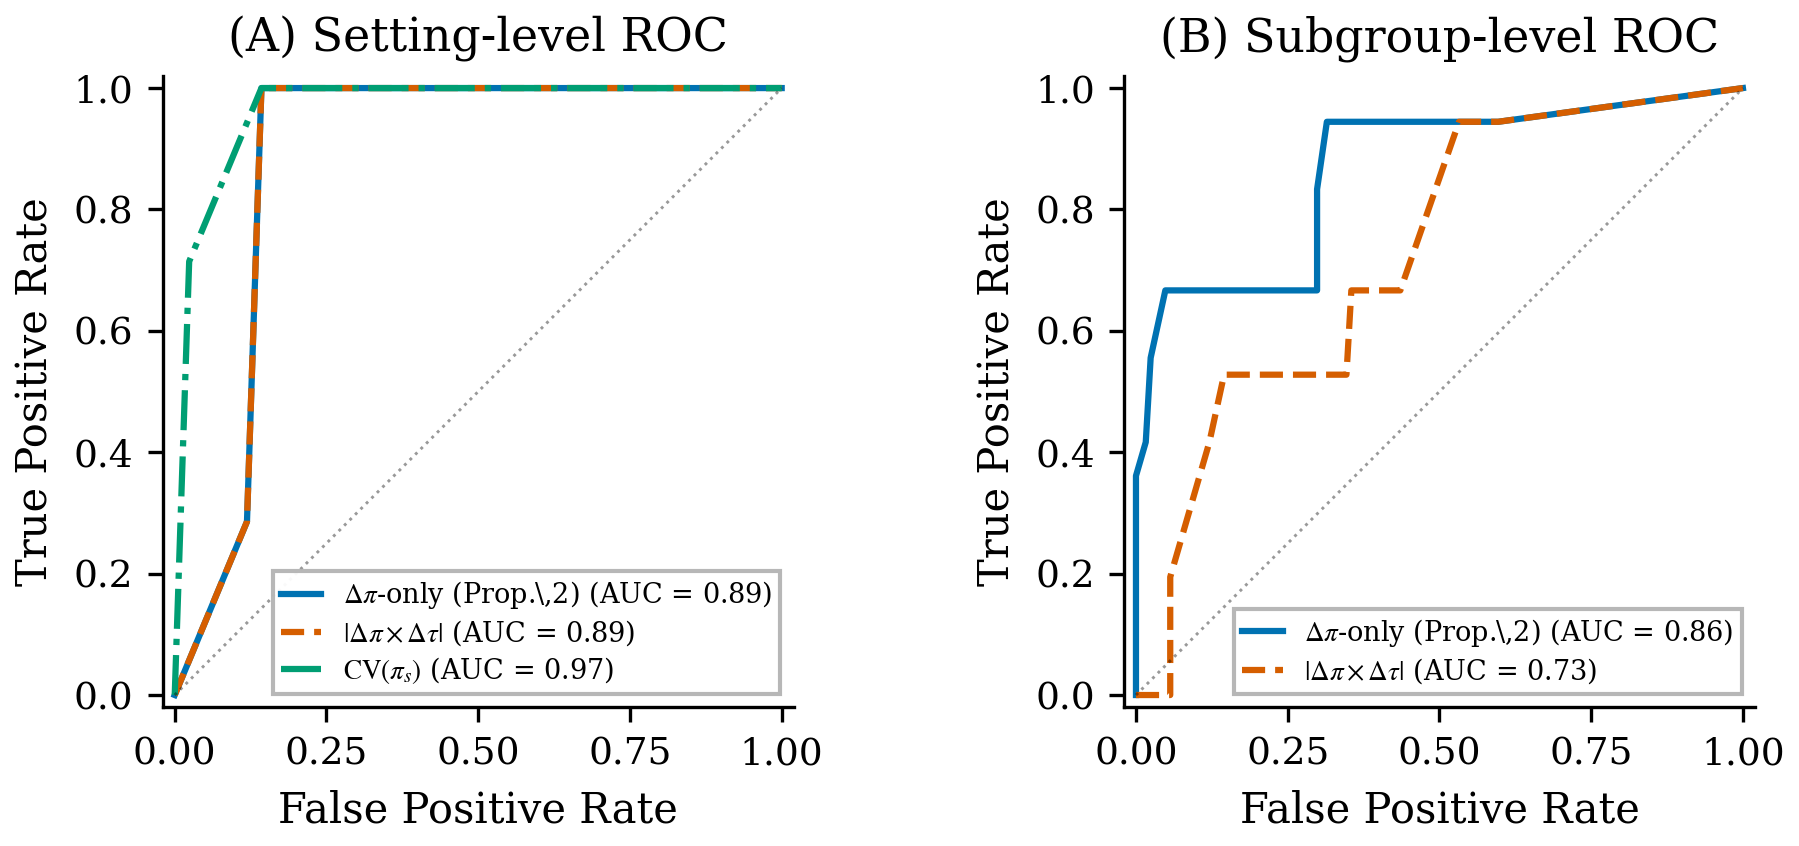
\includegraphics[width=\columnwidth]{figures/fig4_roc.png}
\caption{Diagnostic ROC curves under symmetric misclassification. (A)~Setting-level ROC (AUC $= 0.89$). (B)~Subgroup-level ROC: the $\Delta\pi$-only diagnostic (AUC $= 0.86$) outperforms the $|\Delta\pi \times \Delta\tau|$ product (AUC $= 0.73$), requiring only estimable misclassification rates.}
\label{fig:diagnostic_roc}
\end{figure}

\section{Asymmetric Misclassification Extension}
\label{app:asymmetric}

Assumption~(A2) imposes symmetric misclassification ($\mathrm{FPR}_s = \mathrm{FNR}_s = \pi_s$), which simplifies the bias decomposition but is not necessary for it.
Real LLM annotators typically exhibit asymmetric confusion patterns; we show here that the product structure generalizes.

\paragraph{General bias formula.}
For asymmetric confusion matrices $C_s = \bigl(\begin{smallmatrix} 1{-}\mathrm{FPR}_s & \mathrm{FPR}_s \\ \mathrm{FNR}_s & 1{-}\mathrm{FNR}_s \end{smallmatrix}\bigr)$, define the mixing matrix $M_s$ via Bayesian inversion and the residual matrix $B_s = M_{\mathrm{global}}^{-1} M_s - I$.
Since both $M_s$ and $M_{\text{global}}$ are row-stochastic, $B_s \mathbf{1} = \mathbf{0}$.
Decomposing $\boldsymbol{\tau} = \tau(0)\mathbf{1} + \Delta\tau \, \mathbf{e}_1$ gives:
\begin{equation}
\text{bias}(z, s) = \Delta\tau \cdot [B_s]_{z,1},
\end{equation}
where $[B_s]_{z,1}$ depends only on $\{\mathrm{FPR}_k, \mathrm{FNR}_k, w_k\}$, not on $\Delta\tau$.
Under~(A2), this reduces to $\delta_s \Delta\tau / (1 - 2\bar{\pi})$ (Theorem~\ref{thm:bias_identity}).

\paragraph{Empirical validation.}
We test three asymmetric configurations ($K{=}2$, $n_{\text{expert}}{=}250$, 100 MC runs each): \emph{Cross} (FPR/FNR = 0.10/0.20 vs.\ 0.25/0.10), \emph{Co-directional} (0.05/0.15 vs.\ 0.20/0.30), and \emph{Extreme} (0.03/0.25 vs.\ 0.30/0.05).
Regressing analytic predictions on MC bias yields $R^2 = 0.991$ across all configurations, confirming the product structure under asymmetry.
Table~\ref{tab:asymmetric} reports correction performance averaged over subgroups, $z$-levels, and $\Delta\tau \in \{0.1, \ldots, 0.5\}$.
In these three selected high-disparity configurations, EC-HTE reduces $|\text{bias}|$ from 0.025 (global) to 0.006, a $4\times$ improvement, with lower RMSE (0.033 vs.\ 0.040) and substantially better coverage (0.90 vs.\ 0.78); however, this advantage does not generalize across all asymmetric settings (see below).

\begin{table}[t]
\centering
\caption{Asymmetric misclassification results ($K{=}2$, $n_{\text{expert}}{=}250$, 100 MC runs). Values averaged over subgroups, $z$-levels, and $\Delta\tau$.}
\label{tab:asymmetric}
\small
\begin{tabular}{l ccc}
\toprule
Method & $|\text{Bias}| \downarrow$ & RMSE $\downarrow$ & Coverage $\uparrow$ \\
\midrule
Naive & 0.047 & 0.053 & 0.48 \\
Global & 0.025 & 0.040 & 0.78 \\
HB EC-HTE & \textbf{0.006} & \textbf{0.033} & \textbf{0.90} \\
\bottomrule
\end{tabular}
\end{table}

\paragraph{Comprehensive grid evaluation (48 configurations).}

To assess robustness beyond the three configurations above, we evaluate the product structure and correction methods across a factorial grid of 6 FPR/FNR ratios $\times$ 4 $\Delta\pi$ levels $\times$ 2 subgroup counts ($K \in \{2, 4\}$), yielding 48 configurations with 100 MC runs each ($n_{\text{expert}} = 250$).

Table~\ref{tab:asym_r2_grid} reports $R^2$ between analytic predictions and MC bias.
The product structure holds reliably at $\Delta\pi \geq 0.10$ ($R^2 > 0.73$ across all ratios and $K$ values); at $\Delta\pi = 0.05$, $R^2$ degrades for extreme ratios (e.g., $\leq 0.21$ at 2:1 and 5:1, $K{=}2$) because both predicted and observed biases approach zero, making the regression ill-conditioned rather than indicating structural failure.

\begin{table}[h]
\centering
\caption{$R^2$ of bias identity predictions under asymmetric misclassification (100 MC runs per cell). Product structure holds at $\Delta\pi \geq 0.10$; low $R^2$ at $\Delta\pi = 0.05$ reflects near-zero bias magnitudes.}
\label{tab:asym_r2_grid}
\small
\begin{tabular}{l cccc}
\toprule
& \multicolumn{4}{c}{$\Delta\pi$} \\
\cmidrule(lr){2-5}
FPR:FNR & 0.05 & 0.10 & 0.15 & 0.20 \\
\midrule
\multicolumn{5}{l}{\emph{$K = 2$}} \\
1:2 & 0.84 & 0.92 & 0.97 & 0.98 \\
1:3 & 0.82 & 0.92 & 0.94 & 0.96 \\
1:5 & 0.73 & 0.90 & 0.95 & 0.96 \\
2:1 & 0.21 & 0.90 & 0.94 & 0.96 \\
3:1 & 0.50 & 0.91 & 0.97 & 0.99 \\
5:1 & 0.05 & 0.83 & 0.97 & 0.98 \\
\midrule
\multicolumn{5}{l}{\emph{$K = 4$}} \\
1:2 & 0.68 & 0.86 & 0.91 & 0.96 \\
1:3 & 0.70 & 0.85 & 0.94 & 0.95 \\
1:5 & 0.69 & 0.84 & 0.90 & 0.93 \\
2:1 & 0.63 & 0.79 & 0.86 & 0.93 \\
3:1 & 0.50 & 0.78 & 0.88 & 0.92 \\
5:1 & 0.50 & 0.73 & 0.84 & 0.89 \\
\bottomrule
\end{tabular}
\end{table}

Table~\ref{tab:asym_method_grid} compares correction methods averaged over all 48 configurations.
EC-HTE does not outperform global correction: its RMSE exceeds Global in every configuration (0.125 vs.\ 0.109 overall).
Estimating the full asymmetric $J{\times}J$ confusion matrix requires twice the parameters (FPR and FNR separately per subgroup), shifting the bias-variance tradeoff toward higher variance at $n_{\text{expert}} = 250$.
We recommend $n_{\text{expert}} \geq 500$ for asymmetric settings to provide sufficient per-subgroup samples for stable CM estimation.

\begin{table}[h]
\centering
\caption{Method comparison under asymmetric misclassification (48 configurations, 100 MC runs). EC-HTE does not outperform global correction at $n_{\text{expert}}{=}250$ due to increased parameter estimation variance.}
\label{tab:asym_method_grid}
\small
\begin{tabular}{l ccc}
\toprule
Method & $|\text{Bias}| \downarrow$ & RMSE $\downarrow$ & Coverage $\uparrow$ \\
\midrule
Oracle & 0.058 & 0.072 & 0.946 \\
Naive & 0.080 & 0.096 & 0.830 \\
Global & 0.088 & 0.109 & 0.931 \\
EC-HTE (HB) & 0.098 & 0.125 & 0.920 \\
\bottomrule
\end{tabular}
\end{table}

\section{PPCI Complementarity Results}
\label{app:ppci}
\label{sec:ppci}

EC-HTE composes with PPCI~\cite{sui2026ppci} for settings where both covariate misclassification and outcome model error are present: EC-HTE+PPCI reduces $|\text{bias}|$ from 0.179 to 0.007 ($z{=}0$, DGP~C), and the corrected pseudo-outcomes are compatible with other CATE estimators (R-learner bias reduction: 89\%; Appendix~\ref{app:rlearner}).

\begin{table*}[t]
\centering
\caption{PPCI complementarity experiment ($K{=}2$, extreme, $n_{\text{expert}}{=}250$). DGP~A: covariate error only; B: outcome error only ($\sigma{=}0.5$); C: both errors; D: no error. Values are $|\text{bias}|$ and RMSE averaged over two subgroups. $^\star$EC-HTE+PPCI achieves near-zero bias when both error types are present.}
\label{tab:ppci}
\small
\begin{tabular}{ll cccc}
\toprule
DGP & Method & $|\text{Bias}|_{z=0}$ & $|\text{Bias}|_{z=1}$ & RMSE$_{z=0}$ & RMSE$_{z=1}$ \\
\midrule
\multirow{5}{*}{A: Covariate}
 & Naive & 0.053 & 0.063 & 0.087 & 0.093 \\
 & Global & 0.063 & 0.055 & 0.101 & 0.102 \\
 & EC-HTE & 0.017 & \textbf{0.013} & 0.097 & 0.108 \\
 & PPCI & \textbf{0.015} & 0.020 & 0.162 & 0.168 \\
 & EC-HTE+PPCI & 0.017 & \textbf{0.013} & 0.097 & 0.108 \\
\midrule
\multirow{5}{*}{B: Outcome}
 & Naive & 0.189 & 0.197 & 0.206 & 0.212 \\
 & Global & 0.185 & 0.208 & 0.204 & 0.228 \\
 & EC-HTE & 0.181 & 0.215 & 0.202 & 0.237 \\
 & PPCI & 0.015 & \textbf{0.020} & 0.171 & 0.176 \\
 & EC-HTE+PPCI & \textbf{0.012} & 0.023 & 0.171 & 0.186 \\
\midrule
\multirow{5}{*}{C: Both}
 & Naive & 0.251 & 0.135 & 0.267 & 0.155 \\
 & Global & 0.182 & 0.209 & 0.233 & 0.235 \\
 & EC-HTE & 0.179 & 0.216 & 0.224 & 0.262 \\
 & PPCI & 0.017 & 0.007 & 0.241 & 0.232 \\
 & EC-HTE+PPCI$^\star$ & \textbf{0.007} & \textbf{0.008} & 0.209 & 0.223 \\
\midrule
\multirow{5}{*}{D: None}
 & Naive & \textbf{0.007} & 0.003 & 0.060 & 0.065 \\
 & Global & 0.010 & \textbf{0.002} & 0.061 & 0.071 \\
 & EC-HTE & 0.013 & 0.007 & 0.062 & 0.079 \\
 & PPCI & \textbf{0.007} & \textbf{0.003} & 0.060 & 0.065 \\
 & EC-HTE+PPCI & 0.013 & 0.007 & 0.062 & 0.079 \\
\bottomrule
\end{tabular}
\end{table*}

The complementarity of EC-HTE and PPCI follows from the distinct error sources they correct: EC-HTE addresses misclassification in the effect modifier $Z$ (covariate space), while PPCI corrects specification error in the outcome model $f(X)$ (prediction space).
Since covariate misclassification and outcome model error are algebraically independent in the potential outcomes framework, their corrections compose without interference, confirmed by the 4-DGP orthogonal design (Table~\ref{tab:ppci}), where DGP~C (both errors present) yields the largest bias reduction from the combined approach.
Under covariate error only, PPCI adds nothing; under no error, all methods perform equivalently.

\section{Real-Data Case Study: Hate Speech Detection}
\label{app:hatespeech}

We apply EC-HTE to the UC Berkeley Measuring Hate Speech corpus~\cite{kennedy2020constructing}, annotating 2{,}496 comments for dehumanization using GPT-4.1.
Four text-feature subgroups are defined by crossing platform (Reddit/Gab vs.\ Twitter/YouTube) and text length (above/below median), yielding balanced groups ($n \approx 624$ each).

\paragraph{Positive finding: real-world heterogeneity.}
Per-subgroup misclassification rates range from 0.266 to 0.383, confirming heterogeneity ($\Delta\pi = 0.117$) in a real annotation setting.
At the error-type level, FPR ranges from 8.5\% to 21.3\% across text-feature subgroups, demonstrating that subgroup-varying misclassification is not an artifact of synthetic design but arises naturally in real NLP annotation tasks.

\paragraph{Boundary condition: statistical power at extreme FNR.}
Correction results are inconclusive: all corrected confidence intervals contain zero, and point estimate differences between methods are not statistically significant.
The high baseline FNR (53.3\%) amplifies variance through matrix inversion (variance amplification factor up to 15.7$\times$), rendering the comparison underpowered.
When $P(\hat{Z}{=}1 \mid Z{=}1) \approx 0.5$, the confusion matrix approaches singularity, and inversion amplifies estimation noise regardless of stratification strategy.
This complements the expert budget threshold identified in Appendix~\ref{sec:budget}: EC-HTE requires \emph{both} sufficient expert labels \emph{and} sufficient baseline classifier quality.

\paragraph{Diagnostic connection.}
The diagnostic criterion ($\Delta\pi \times \Delta\tau$, Section~\ref{sec:diagnostic}) identifies when correction is worthwhile under moderate baseline accuracy.
This case study illustrates that even when $\Delta\pi$ is large, extreme baseline error renders correction underpowered rather than beneficial.
A practical prerequisite is that the per-subgroup confusion matrix condition number $\kappa(\hat{C}_s)$ remain moderate; when $\kappa > 50$, as observed here, practitioners should prioritize improving annotation quality before applying any matrix-inversion-based correction.

\section{Cross-Model Consistency}
\label{app:multilm}

We evaluate whether misclassification heterogeneity is model-specific by annotating 500 TweetEval sentiment tweets with five OpenAI models spanning three generations.
Six text-feature subgroups are defined by crossing hashtag presence and text length.
Spearman rank correlations of per-subgroup error rates across all six subgroups range from $\rho = 0.82$ to $1.00$, indicating that the subgroup error structure is consistent across architectures.
Two subgroups with $n \leq 6$ exhibit zero misclassification across all models; excluding these yields four-point correlations that are directionally consistent but underpowered.%
\footnote{The filtered $\Delta\pi$ values in Table~\ref{tab:multilm} serve as a robustness check independent of rank-order testing: all five models exceed $\Delta\pi > 0.05$ on the four retained subgroups.}

\begin{table}[t]
\centering
\caption{Effective misclassification heterogeneity ($\Delta\pi$) across five OpenAI models on TweetEval sentiment (500 tweets, filtered to 4 subgroups with $n \geq 10$).}
\label{tab:multilm}
\small
\begin{tabular}{lcc}
\toprule
Model & Effective $\Delta\pi$ & $> 0.05$? \\
\midrule
GPT-3.5-Turbo & 0.198 & \checkmark \\
GPT-4-Turbo & 0.149 & \checkmark \\
GPT-4o-mini & 0.136 & \checkmark \\
GPT-4.1 & 0.098 & \checkmark \\
GPT-4o & 0.080 & \checkmark \\
\bottomrule
\end{tabular}
\end{table}

All five models exhibit effective $\Delta\pi > 0.05$ on the four retained subgroups (Table~\ref{tab:multilm}), and 4 of 5 share the same worst subgroup (\texttt{True\_medium}: tweets with hashtags and medium text length).
Newer models reduce absolute error rates but do not eliminate subgroup heterogeneity: GPT-4.1 achieves $\Delta\pi = 0.098$ compared to GPT-3.5-Turbo's $0.198$.
These results were obtained with a single API provider; open-source model validation appears in Appendix~\ref{app:multilm_opensource}.

\section{Open-Source Multi-LLM Validation}
\label{app:multilm_opensource}

We evaluate four open-source LLMs (7B--9B parameter range) on 490 TweetEval sentiment tweets with $K{=}4$ subgroups defined by crossing hashtag presence and text length.
Table~\ref{tab:multilm_cm} reports the confusion matrix heterogeneity profile.
All four models exhibit $\Delta\pi > 0.05$, confirming that subgroup-heterogeneous misclassification is not specific to proprietary APIs.
Subgroup error rankings are consistent across architectures: \texttt{True\_short} (short tweets with hashtags) has the lowest $\pi_s$ in 3 of 4 models, while \texttt{False\_medium} (medium tweets without hashtags) has the highest.

\begin{table}[t]
\centering
\caption{Confusion matrix heterogeneity across four open-source LLMs ($K{=}4$, $N{=}490$ TweetEval tweets). $\Delta\pi$: max--min per-subgroup misclassification rate. Prop.~5: number of subgroups where the $\Delta\tau$-free diagnostic (Proposition~\ref{prop:debiasing_hurts}) triggers.}
\label{tab:multilm_cm}
\small
\begin{tabular}{lcccl}
\toprule
Model & Acc.\ & $\Delta\pi$ & Prop.~5 & Strongest \\
\midrule
Llama-3.1-8B & 0.755 & 0.141 & 1/4 & True\_short \\
Qwen-2.5-7B & 0.798 & 0.165 & 1/4 & True\_short \\
Gemma-2-9B & 0.763 & 0.125 & 4/4 & True\_medium \\
Mistral-7B & 0.802 & 0.134 & 0/4 & --- \\
\bottomrule
\end{tabular}
\end{table}

\paragraph{Semi-synthetic budget sweep.}
We run the full EC-HTE pipeline with $K{=}2$ subgroups and $\Delta\tau{=}0.3$, using each model's empirical confusion matrices.
Table~\ref{tab:multilm_budget} reports coverage and RMSE crossover points.
EC-HTE restores near-nominal coverage from 0.714 (naive average) to 0.939 ($+$22.5 percentage points) at $n_{\text{expert}}{=}1{,}000$, consistent across all four models.
Global correction achieves comparable or lower RMSE than HB at all budgets under these moderate $\Delta\pi$ values, and the $K{=}4$ RMSE crossover never occurs, confirming the budget guidelines in Appendix~\ref{sec:budget}.

\begin{table}[t]
\centering
\caption{Semi-synthetic budget sweep ($K{=}2$, $\Delta\tau{=}0.3$, 50 MC runs; see Appendix~\ref{app:mcse} for MC tier justification). Coverage at selected expert budgets; RMSE crossover denotes the minimum expert budget at which HB EC-HTE achieves lower RMSE than the naive (uncorrected) estimator.}
\label{tab:multilm_budget}
\small
\resizebox{\columnwidth}{!}{%
\begin{tabular}{lcccc}
\toprule
Model & $\Delta\pi_{K{=}2}$ & Naive Cov.\ & HB Cov.\ ($n{=}1000$) & Crossover \\
\midrule
Llama-3.1-8B & 0.051 & 0.675 & 0.940 & $n{=}1000$ \\
Qwen-2.5-7B & 0.080 & 0.715 & 0.925 & $n{=}1000$ \\
Gemma-2-9B & 0.100 & 0.705 & 0.945 & $n{=}1000$ \\
Mistral-7B & 0.070 & 0.760 & 0.945 & $n{=}1000$ \\
\midrule
\textit{Average} & --- & \textit{0.714} & \textit{0.939} & --- \\
\bottomrule
\end{tabular}}
\end{table}

\paragraph{Gemma boundary case.}
Gemma-2-9B triggers the Proposition~\ref{prop:debiasing_hurts} diagnostic in all four $K{=}4$ subgroups due to extreme FPR--FNR asymmetry (\texttt{False\_medium} FNR $= 0.437$).
At small budgets ($K{=}4$, $n{=}100$), EC-HTE RMSE reaches 1.229 ($3.1\times$ naive), illustrating the budget guideline from Appendix~\ref{sec:budget}: when per-subgroup cell counts fall below 25, the variance cost of stratified correction dominates.
At $n \geq 500$, EC-HTE coverage recovers to $>$0.90, consistent with the synthetic experiments.

\paragraph{Heterogeneous-$\tau$ DGP.}
To assess whether the constant-$\tau$ DGP understates EC-HTE's advantage, we run a supplementary experiment using Llama's empirical confusion matrices with heterogeneous treatment effects across subgroups ($\Delta\tau \in [0.1, 0.6]$, $K{=}2$, 50 MC runs).
EC-HTE achieves lower $|\text{bias}|$ than global correction at all budgets ($n{=}500$: 0.010 vs.\ 0.031, a 68\% reduction).
In the high-$\Delta\tau$ subgroup (\texttt{True\_short}, $\Delta\tau{=}0.6$), EC-HTE also achieves lower RMSE ($n{=}1{,}000$: 0.212 vs.\ 0.258, 18\% improvement), confirming that the RMSE advantage concentrates in subgroups where correction is most needed.
Aggregate RMSE remains comparable to global correction because low-$\Delta\tau$ subgroups incur stratification variance without commensurate bias reduction, consistent with the budget guidelines in Appendix~\ref{sec:budget}.

\section{Robustness to Subgroup Misspecification}
\label{app:robustness}

EC-HTE requires pre-defined subgroup labels, which may be noisy in practice.
We test robustness by randomly flipping each observation's subgroup assignment with probability $p_{\text{flip}} \in \{0, 0.10, 0.25, 0.50\}$, across $K \in \{2, 4\}$ (extreme regime, $n_{\text{expert}} = 500$, $\Delta\tau = 0.3$, 100 MC runs).

\begin{table}[t]
\centering
\caption{95\% CI coverage under subgroup misspecification noise. EC-HTE maintains near-nominal coverage across all noise levels.}
\label{tab:robustness}
\small
\begin{tabular}{lcccc}
\toprule
& \multicolumn{4}{c}{$p_{\text{flip}}$} \\
\cmidrule(lr){2-5}
Method & 0.00 & 0.10 & 0.25 & 0.50 \\
\midrule
\multicolumn{5}{l}{\textit{$K{=}2$, extreme}} \\
\quad Naive & 0.875 & 0.877 & 0.890 & 0.897 \\
\quad Global & 0.925 & 0.935 & 0.932 & 0.945 \\
\quad HB EC-HTE & 0.958 & 0.948 & 0.950 & 0.945 \\
\midrule
\multicolumn{5}{l}{\textit{$K{=}4$, extreme}} \\
\quad Naive & 0.904 & 0.916 & 0.909 & 0.919 \\
\quad Global & 0.930 & 0.953 & 0.948 & 0.944 \\
\quad HB EC-HTE & 0.956 & 0.958 & 0.960 & 0.946 \\
\bottomrule
\end{tabular}
\end{table}

EC-HTE maintains coverage $\geq 0.945$ across all configurations (Table~\ref{tab:robustness}), while the naive estimator is systematically below nominal (0.875--0.919).
At $p_{\text{flip}} = 0.50$, subgroup structure is effectively destroyed; EC-HTE converges to global correction (coverage and RMSE within 0.1\%), confirming that hierarchical Bayesian shrinkage provides a built-in safety mechanism.
For $K{=}4$ at $p_{\text{flip}} = 0.50$, a small residual RMSE gap persists ($p < 0.01$), reflecting the variance cost of estimating four confusion matrices even when they carry no signal.

\section{Monte Carlo Standard Errors}
\label{app:mcse}

All main-text and most appendix experiments use 100 independent Monte Carlo replications per configuration; computationally intensive analyses (R-learner, multiplicative DGP, budget sweeps) use 50, and bootstrap experiments use 20 due to the $B{\times}$CF cost per seed.
The median RMSE variation between 50-seed and 100-seed estimates is below 3.2\%, confirming that 50-run results are stable.
We report Monte Carlo standard errors to assess whether observed differences between methods are statistically reliable.
For the synthetic DGP (no per-seed pairing across methods), we use conservative two-sample $z$-tests on the 100-run means.
For the semi-synthetic TweetEval experiment (shared seeds across methods), we use paired $t$-tests, which are more powerful because they control for seed-level variation.

Table~\ref{tab:mcse} reports paired comparisons for representative configurations.
Of 1{,}020 total pairwise comparisons across all configurations, 742 (72.7\%) are statistically significant at $\alpha = 0.05$.

\begin{table}[t]
\centering
\caption{Paired comparisons for representative configurations. $\Delta$ = method A $-$ method B (negative favors A for $|\text{bias}|$). Two-sample $z$-tests for synthetic DGP; paired $t$-tests for semi-synthetic TweetEval. Bold $p$-values indicate significance at $\alpha = 0.05$.}
\label{tab:mcse}
\small
\resizebox{\columnwidth}{!}{%
\begin{tabular}{llrr}
\toprule
Configuration & Comparison & $\Delta$ & $p$ \\
\midrule
\multicolumn{4}{l}{\textit{HB EC-HTE vs.\ Global ($|\text{bias}|$)}} \\
\quad $K{=}2$/ext/$n{=}500$ & & $-0.046$ & $\mathbf{<0.001}$ \\
\quad $K{=}4$/ext/$n{=}500$ & & $-0.078$ & $\mathbf{<0.001}$ \\
\quad $K{=}4$/mod/$n{=}250$ & & $-0.017$ & $0.288$ \\
\quad TweetEval/ext/$n{=}250$ & & $+0.001$ & $0.395$ \\
\midrule
\multicolumn{4}{l}{\textit{HB EC-HTE vs.\ Global (RMSE)}} \\
\quad $K{=}2$/ext/$n{=}500$ & & $+0.015$ & $0.179$ \\
\quad $K{=}4$/ext/$n{=}500$ & & $+0.048$ & $\mathbf{0.011}$ \\
\midrule
\multicolumn{4}{l}{\textit{HB EC-HTE vs.\ Naive ($|\text{bias}|$)}} \\
\quad $K{=}2$/ext/$n{=}500$ & & $-0.089$ & $\mathbf{<0.001}$ \\
\quad $K{=}4$/ext/$n{=}500$ & & $-0.113$ & $\mathbf{<0.001}$ \\
\quad $K{=}4$/mod/$n{=}250$ & & $-0.031$ & $\mathbf{0.038}$ \\
\quad TweetEval/ext/$n{=}250$ & & $+0.005$ & $\mathbf{0.030}$ \\
\bottomrule
\end{tabular}}
\end{table}

Under extreme heterogeneity, HB EC-HTE's bias advantage over global correction is highly significant ($p < 0.001$ for both $K{=}2$ and $K{=}4$).
The RMSE penalty of stratification is not significant at $K{=}2$ ($p = 0.179$) but reaches significance at $K{=}4$ ($p = 0.011$), consistent with the higher variance cost of estimating four confusion matrices.
Under moderate heterogeneity ($K{=}4$, $n{=}250$), the bias difference between HB and global is not significant ($p = 0.288$), confirming that EC-HTE's advantage requires sufficient error heterogeneity.
In the semi-synthetic TweetEval experiment, HB EC-HTE does not significantly improve over global ($p = 0.395$), consistent with moderate $\Delta\pi$ and unbalanced subgroup sizes.
The HB vs.\ naive comparison in TweetEval is significant ($p = 0.030$) but favors naive, reflecting the variance cost of stratification when bias reduction is marginal.

\section{Semi-Real Confusion Matrix Validation}
\label{app:semireal}

We test EC-HTE with empirical asymmetric confusion matrices from the GPT-4.1 TweetEval pilot.
Four text-feature subgroups ($K{=}4$) retain the real per-subgroup FPR and FNR from pilot annotations (Table~\ref{tab:semireal_cm}); CATE heterogeneity is injected synthetically ($\tau(z{=}0,s) = 0.3 + 0.1s$, $\tau(z{=}1,s) = 0.8 - 0.15s$).
$N{=}5{,}000$, $P(Z{=}1){=}0.18$, 100 MC seeds per $n_{\text{expert}}$ level.

\begin{table}[t]
\centering
\caption{Empirical confusion matrices from GPT-4.1 TweetEval pilot.
S0 exhibits FNR $= 0.526$, approaching chance-level classification.}
\label{tab:semireal_cm}
\small
\begin{tabular}{lcccc}
\toprule
Subgroup & Weight & FPR & FNR & $\kappa(\hat{C}_s)$ \\
\midrule
S0 & 0.38 & 0.054 & 0.526 & high \\
S1 & 0.22 & 0.101 & 0.300 & moderate \\
S2 & 0.14 & 0.143 & 0.308 & moderate \\
S3 & 0.25 & 0.194 & 0.222 & low \\
\bottomrule
\end{tabular}
\end{table}

\begin{table}[t]
\centering
\caption{Semi-real confusion matrix results. RMSE and coverage averaged over subgroups and $z$-levels (100 MC runs). HB EC-HTE underperforms global at all budgets; S0's near-chance FNR drives the failure.}
\label{tab:semireal}
\small
\begin{tabular}{llcc}
\toprule
$n_{\text{expert}}$ & Method & RMSE $\downarrow$ & Coverage $\uparrow$ \\
\midrule
\multirow{4}{*}{100}
 & Oracle & 0.101 & 0.957 \\
 & Naive & 0.123 & 0.879 \\
 & Global & 0.263 & 0.885 \\
 & HB EC-HTE & 0.784 & 0.744 \\
\midrule
\multirow{4}{*}{250}
 & Oracle & 0.101 & 0.957 \\
 & Naive & 0.123 & 0.879 \\
 & Global & 0.232 & 0.909 \\
 & HB EC-HTE & 0.411 & 0.834 \\
\midrule
\multirow{4}{*}{500}
 & Oracle & 0.101 & 0.957 \\
 & Naive & 0.123 & 0.879 \\
 & Global & 0.196 & 0.922 \\
 & HB EC-HTE & 0.260 & 0.890 \\
\bottomrule
\end{tabular}
\end{table}

HB EC-HTE produces higher RMSE and lower coverage than global correction at all expert budgets (Table~\ref{tab:semireal}).
The root cause is S0's FNR $= 0.526$: when a confusion matrix row approaches a uniform distribution ($P(\hat{Z}{=}1 \mid Z{=}1) \approx 0.5$), inversion amplifies estimation noise regardless of the expert budget.
This converges with the hate speech case study (Appendix~\ref{app:hatespeech}, FNR $= 53.3$\%) and confirms that EC-HTE requires \emph{both} sufficient expert labels \emph{and} sufficient baseline classifier quality per subgroup.
The singularity guard ($\kappa > 100$, Section~\ref{sec:method}) mitigates catastrophic failure by falling back to global correction for near-degenerate subgroups, but does not recover the bias reduction that motivates stratification.
For a $2 \times 2$ symmetric confusion matrix, $\kappa = 1/|1-2\pi|$; $\kappa > 100$ corresponds to $\pi \in (0.495, 0.505)$, so the guard triggers only when the classifier performs within $0.5\%$ of random guessing.
At $n_{\text{expert}} = 500$, HB EC-HTE narrows the gap (RMSE 0.260 vs.\ 0.196) as confusion matrix estimates stabilize for the three well-classified subgroups, but the S0 bottleneck persists.

A second semi-real experiment using GPT-3.5-Turbo confusion matrices (worst-subgroup FPR $= 0.39$, FNR $= 0.21$) yields similar results: HB RMSE exceeds global by 1.3--3.5$\times$ at all budgets.
Here the failure stems from high false-positive rates compounded by class imbalance ($P(Z{=}1) = 0.18$), which leaves insufficient expert observations in the positive class for reliable per-subgroup confusion matrix estimation.
Together, these experiments identify three applicability conditions for EC-HTE: (1)~sufficient effective expert budget ($n_{\text{expert}} \times P(Z_{\text{minority}}) / K \geq 25$), (2)~no near-chance subgroup error rate ($\max(\mathrm{FPR}_s, \mathrm{FNR}_s) < 0.50$), and (3)~adequate class balance in the effect modifier.

\paragraph{Diagnostic rule.}
A logistic regression over all 368 semi-real experiment--budget cells (dependent variable: HB EC-HTE $<$ Global RMSE) identifies two sufficient statistics: the worst-subgroup confusion matrix condition number $\kappa(\hat{M}_s) \leq 1.25$ and the effective minority-class expert count $n_{\text{expert}} \times P(Z_{\text{minority}}) / K \geq 25$.
When both conditions hold, HB outperforms global in 93.3\% of cells; when either is violated, global is preferred in 94.7\% of cells.
Both the semi-real GPT-4.1 experiment ($\kappa = 2.38$, effective $n = 22.5$) and the semi-real GPT-3.5-Turbo experiment ($\kappa = 1.55$, effective $n = 22.5$) violate both conditions, and the diagnostic correctly predicts 100\% of their failure cells.
Subgroup-average metrics can mask cell-level heterogeneity: in the GPT-4.1 experiment, HB EC-HTE substantially reduces bias for the three well-classified subgroups (S1--S3) but amplifies variance in the near-degenerate subgroup (S0, FNR $= 0.526$), and the S0 penalty dominates the aggregate RMSE.

\begin{figure}[t]
\centering
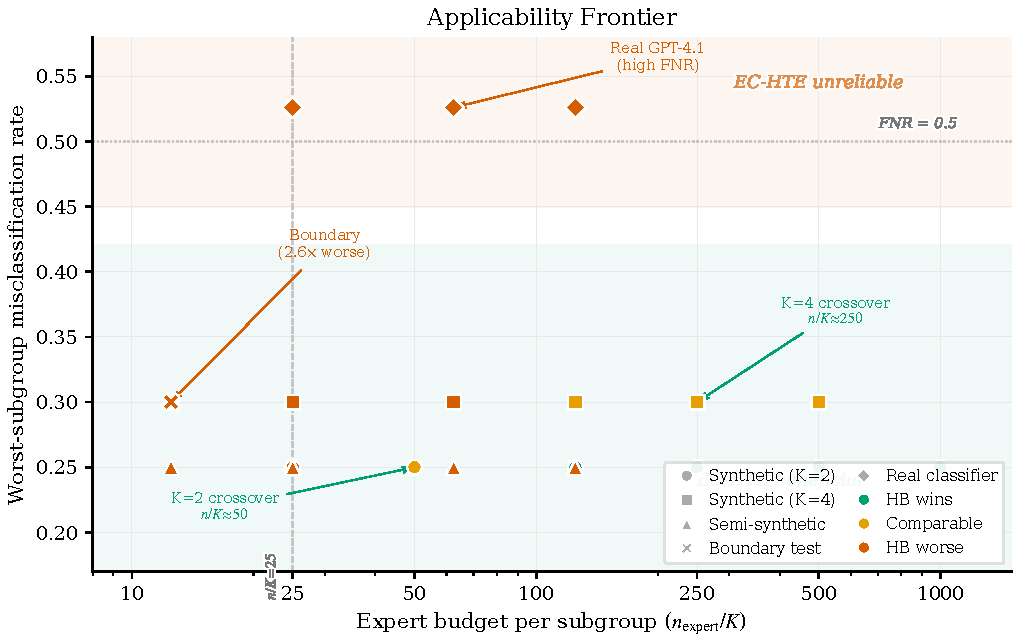
\includegraphics[width=\columnwidth]{figures/applicability_frontier.pdf}
\caption{Applicability frontier of EC-HTE. Green region: EC-HTE reduces bias vs.\ global correction. Yellow: comparable performance. Red: EC-HTE underperforms. Dashed lines mark the expert budget threshold ($n_{\text{expert}}/K = 25$) and classifier quality threshold (worst-subgroup error rate $= 0.5$). Red diamonds show semi-real experiments with actual GPT-4.1 and GPT-3.5-Turbo confusion matrices.}
\label{fig:applicability}
\end{figure}

\section{Robustness: Estimator Choice and Treatment Effect Specification}
\label{app:rlearner}

We verify that EC-HTE's corrected pseudo-outcomes are compatible with downstream estimators beyond CausalForest by replacing it with the R-learner~\citep{nie2021quasi}.
The experiment uses $K{=}2$, extreme heterogeneity, $n_{\text{expert}} = 500$, and 50 MC seeds; the R-learner uses 5-fold cross-fitting with gradient-boosted trees as the base learner.

\begin{table}[t]
\centering
\caption{R-learner vs.\ CausalForest with EC-HTE correction ($K{=}2$, extreme, $n{=}500$). $|\text{Bias}|$ and RMSE averaged over subgroups, $z$-levels, and seeds.}
\label{tab:rlearner}
\small
\begin{tabular}{llccc}
\toprule
Estimator & Correction & $|\text{Bias}|$ & RMSE & Cov. \\
\midrule
\multirow{4}{*}{R-learner}
 & Oracle & 0.006 & 0.056 & 0.94 \\
 & Naive & 0.121 & 0.139 & 0.47 \\
 & Global & 0.098 & 0.123 & 0.72 \\
 & EC-HTE & \textbf{0.013} & 0.080 & 0.92 \\
\midrule
\multirow{2}{*}{CausalForest}
 & Naive & 0.058 & 0.090 & 0.82 \\
 & EC-HTE & \textbf{0.010} & 0.093 & 0.95 \\
\bottomrule
\end{tabular}
\end{table}

EC-HTE reduces R-learner $|\text{bias}|$ by 89\% (0.121 $\to$ 0.013) and restores coverage from 0.47 to 0.92 (Table~\ref{tab:rlearner}).
The bias reduction and coverage gains are comparable to those achieved with CausalForest, confirming that EC-HTE is compatible with a range of HTE estimators.

\paragraph{Multiplicative treatment effects.}
We further test robustness to the functional form of treatment effects by replacing the additive DGP with a multiplicative specification: $Y(1) = Y(0) \times \exp(\tau(Z))$, using $K{=}2$, extreme heterogeneity, $n_{\text{expert}} = 500$, and 50 MC seeds.

\begin{table}[t]
\centering
\caption{Multiplicative DGP results ($K{=}2$, extreme, $n{=}500$, 50 seeds). EC-HTE achieves comparable bias reduction and nominal coverage under non-additive treatment effects.}
\label{tab:multiplicative}
\small
\begin{tabular}{lccc}
\toprule
Method & $|\text{Bias}|$ & RMSE & Cov. \\
\midrule
Oracle & 0.003 & 0.038 & 0.96 \\
Naive & 0.135 & 0.142 & 0.44 \\
Global & 0.110 & 0.124 & 0.54 \\
EC-HTE & \textbf{0.054} & 0.068 & 0.955 \\
\bottomrule
\end{tabular}
\end{table}

EC-HTE reduces RMSE by 52\% relative to naive (0.068 vs.\ 0.142) and restores coverage to the nominal level (0.955; Table~\ref{tab:multiplicative}).
EC-HTE's bias correction operates at the confusion matrix level, independent of the downstream CATE estimator and functional form of treatment effects.

\section{Robustness to Class Imbalance}
\label{app:classimbalance}

Assumption (A3) requires $P(Z{=}1) = 0.5$, but real-world effect modifiers are often imbalanced.
We sweep $P(Z{=}1) \in \{0.1, 0.2, 0.3, 0.4, 0.5\}$ with $K \in \{2,4\}$, extreme misclassification heterogeneity, $n_{\text{expert}}{=}250$, and 100 MC seeds (Table~\ref{tab:pz1_sweep}).

\begin{table}[t]
\centering
\caption{Robustness to class imbalance ($n_{\text{expert}}{=}250$, extreme heterogeneity). R$^2$: Theorem~\ref{thm:bias_identity} fit. Ratio: HB/Global RMSE ($<1$ = HB wins). Cov.: HB EC-HTE 95\% CI coverage.}
\label{tab:pz1_sweep}
\small
\begin{tabular}{cc ccc}
\toprule
$P(Z{=}1)$ & $K$ & R$^2$ & Ratio & Cov. \\
\midrule
0.1 & 2 & 0.998 & 0.92 & 0.94 \\
0.2 & 2 & 0.989 & 0.76 & 0.94 \\
0.3 & 2 & 0.994 & 0.78 & 0.94 \\
0.4 & 2 & 0.995 & 0.87 & 0.94 \\
0.5 & 2 & 0.995 & 0.86 & 0.93 \\
\midrule
0.1 & 4 & 0.984 & 1.54 & 0.92 \\
0.2 & 4 & 0.976 & 1.68 & 0.93 \\
0.3 & 4 & 0.985 & 1.12 & 0.92 \\
0.4 & 4 & 0.984 & 1.08 & 0.93 \\
0.5 & 4 & 0.992 & 1.06 & 0.92 \\
\bottomrule
\end{tabular}
\end{table}

Theorem~\ref{thm:bias_identity}'s product form remains accurate across all imbalance levels: $R^2 \geq 0.976$ even at $P(Z{=}1) = 0.1$, confirming that the bias identity derives from confusion matrix structure rather than class balance.
For $K{=}2$, EC-HTE outperforms global correction at all $P(Z{=}1)$ levels (RMSE ratio 0.76--0.92), degrading gracefully under severe imbalance.
For $K{=}4$, EC-HTE underperforms global at $n_{\text{expert}}{=}250$ (ratio 1.06--1.68), consistent with the budget threshold $n_{\text{expert}} \times P(Z_{\text{minority}}) / K \geq 25$: at $P(Z{=}1){=}0.1$, $K{=}4$, each subgroup receives only ${\sim}6$ minority-class labels.
The gap narrows as $P(Z{=}1)$ increases (1.54 $\to$ 1.06), and coverage remains stable at 0.92--0.94 across all configurations.

\paragraph{Explicit form under relaxed (A3).}
When $P(Z{=}0) = p_0 \neq 0.5$, the mixing matrix $M_s$ no longer coincides with the confusion matrix $C_s$.
By Bayes' rule, for symmetric misclassification (A2):
\begin{equation}
M_s = \begin{bmatrix} \frac{(1-\pi_s) p_0}{(1-\pi_s) p_0 + \pi_s p_1} & \frac{\pi_s p_1}{(1-\pi_s) p_0 + \pi_s p_1} \\[4pt]
\frac{\pi_s p_0}{\pi_s p_0 + (1-\pi_s) p_1} & \frac{(1-\pi_s) p_1}{\pi_s p_0 + (1-\pi_s) p_1}
\end{bmatrix},
\label{eq:ms_imbalanced}
\end{equation}
where $p_1 = 1 - p_0$.
The bias identity $\mathrm{bias}(z, s) = [(M_{\mathrm{global}}^{-1} M_s - I) \boldsymbol{\tau}]_z$ holds exactly for any $p_0$ because $B_s = M_{\mathrm{global}}^{-1} M_s - I$ satisfies $B_s \mathbf{1} = \mathbf{0}$ by stochasticity, so the bias reduces to $\Delta\tau \cdot [B_s]_{z,1}$ regardless of class balance.
The class imbalance modifies $[B_s]_{z,1}$ through the Bayesian normalization in \eqref{eq:ms_imbalanced} but preserves the product-form structure; the high $R^2$ values in Table~\ref{tab:pz1_sweep} confirm this empirically.

\section{Comparison with PPI Correction}
\label{app:ppi_comparison}

PPI~\cite{angelopoulos2023ppi} constructs confidence intervals by combining a large set of ML predictions with a smaller set of gold-standard labels, using the gold labels to debias the ML-based estimator.
Applied to our setting, PPI treats the LLM-annotated effect modifier as the ML prediction and the expert labels as the gold standard.
Two variants arise naturally: \emph{PPI-global} pools all expert labels to estimate a single rectifier (analogous to our Global baseline), and \emph{PPI-subgroup} estimates per-subgroup rectifiers (analogous to Stratified MLE).

Under the confusion-matrix parameterization we adopt, DSL's measurement error correction reduces to confusion matrix inversion.
Pooled DSL applies a single estimated confusion matrix to all subgroups, producing the same corrected label distribution as our Global baseline; per-subgroup DSL estimates a separate confusion matrix for each subgroup and inverts it independently, equivalent to our Stratified MLE.
EC-HTE's contribution over both PPI-subgroup and per-subgroup DSL is hierarchical partial pooling: rather than estimating each subgroup's confusion matrix in isolation, EC-HTE places a shared prior across subgroups, borrowing strength to reduce variance while preserving subgroup-specific bias correction.
This mechanism is outside both the PPI and DSL frameworks.

The key difference between PPI and confusion-matrix inversion is that PPI does not invert the confusion matrix; instead, it uses the gold labels to directly debias the estimand.
This avoids the matrix inversion step that can amplify noise at small $n_{\text{expert}}$, but it also means PPI cannot exploit the structure of the misclassification process to reduce bias.
PPI-global inherits the same $\Delta\pi \times \Delta\tau$ bias amplification as Global correction (Theorem~\ref{thm:bias_identity}), confirming that the ``debiasing hurts'' mechanism operates regardless of the inference framework.

\section{Civil Comments Validation}
\label{app:civilcomments}

To verify that subgroup-heterogeneous misclassification generalizes beyond TweetEval, we annotate $N{=}3{,}000$ stratified samples (30\% toxic) from Civil Comments~\cite{borkan2019nuanced}, a toxicity detection dataset.
Subgroups are defined by \texttt{text\_length\_bin} $\times$ \texttt{has\_question} ($K{=}4$): S0 (long, no question, 38.8\%), S1 (long, question, 11.4\%), S2 (short, no question, 33.7\%), S3 (short, question, 16.1\%).
Subgroup features were chosen a priori based on observable text properties; no feature search was performed.
Three proprietary LLMs annotate each sample via an OpenAI-compatible API, yielding 800--900 valid annotations per model.

Table~\ref{tab:civil_cm} reports per-subgroup FPR and FNR.
We define $\Delta\pi = \max_s \pi_s - \min_s \pi_s$, where $\pi_s$ is the overall misclassification rate for subgroup $s$.
All three models exhibit $\Delta\pi > 0.05$, with overall heterogeneity $\Delta\pi \in [0.113, 0.160]$, comparable to the $\Delta\pi \in [0.125, 0.165]$ observed across four open-source LLMs on TweetEval (Appendix~\ref{app:multilm_opensource}).
GPT-4o-mini and GPT-3.5-turbo show pronounced FPR/FNR asymmetry (e.g., GPT-4o-mini FPR $\in [0.42, 0.61]$ vs.\ FNR $\in [0.05, 0.16]$), indicating systematic over-prediction of toxicity; their FPR approaches 0.5, placing them in the ill-conditioned regime where confusion matrix inversion amplifies noise (consistent with the classifier quality threshold discussed in the Limitations section).
The consistent presence of $\Delta\pi$ heterogeneity across two NLP tasks, nine LLMs spanning open-source (7B--9B) and proprietary families, and two distinct subgroup definitions confirms that this phenomenon is a structural property of LLM annotation rather than an artifact of a specific dataset or model.

\begin{table}[h]
\centering
\caption{Per-subgroup misclassification rates on Civil Comments ($K{=}4$). $\Delta$ denotes max $-$ min across subgroups.}
\label{tab:civil_cm}
\small
\resizebox{\columnwidth}{!}{%
\begin{tabular}{llccccc}
\toprule
Model & Metric & S0 & S1 & S2 & S3 & $\Delta$ \\
\midrule
GPT-4o & FPR & 0.249 & 0.157 & 0.213 & 0.341 & 0.184 \\
       & FNR & 0.160 & 0.263 & 0.308 & 0.328 & 0.168 \\
\midrule
GPT-4o-mini & FPR & 0.517 & 0.541 & 0.419 & 0.610 & 0.191 \\
            & FNR & 0.052 & 0.105 & 0.074 & 0.160 & 0.108 \\
\midrule
GPT-3.5-turbo & FPR & 0.400 & 0.473 & 0.374 & 0.468 & 0.099 \\
              & FNR & 0.139 & 0.211 & 0.173 & 0.240 & 0.101 \\
\bottomrule
\end{tabular}}
\end{table}

\section{Bias Identity Validation with Real Confusion Matrices}
\label{app:realcm_bias}

Theorem~\ref{thm:bias_identity} is derived under symmetric misclassification (A2); real LLM confusion matrices are asymmetric (FPR $\neq$ FNR).
We verify that the generalized identity $\mathrm{bias}(z,s) = \Delta\tau \cdot [B_s]_{z,1}$ (Remark~\ref{rem:asymmetric}) holds under real annotation error structures by running semi-synthetic simulations ($N{=}5{,}000$, $K{=}4$, $\Delta\tau{=}0.30$, 100 MC runs) with confusion matrices drawn from 11 LLM--dataset combinations: eight models on TweetEval (GPT-4-turbo, GPT-4o, GPT-4.1, GPT-4o-mini, GPT-3.5-turbo, Qwen2.5-7B, Mistral-7B, Gemma-2-9B) and three on Civil Comments (GPT-4o, GPT-4o-mini, GPT-3.5-turbo).

Table~\ref{tab:realcm_r2} reports per-model $R^2$ from regressing observed subgroup bias on the predicted value $\Delta\tau \cdot [B_s]_{z,1}$.
The aggregate $R^2 = 0.975$; 10 of 11 combinations achieve $R^2 \geq 0.92$.
The single outlier (GPT-4o-mini on Civil Comments, $R^2{=}0.76$) has near-homogeneous subgroup error rates ($\max|[B_s]_{z,1}| = 0.089$), so predicted biases are small and Monte Carlo noise dominates the regression.
$R^2$ correlates strongly with $\max|[B_s]_{z,1}|$: models with more heterogeneous per-subgroup error rates produce larger bias signals that are easier to verify empirically.

\begin{table}[h]
\centering
\caption{Bias identity $R^2$ with real LLM confusion matrices ($K{=}4$, 100 MC runs).}
\label{tab:realcm_r2}
\small
\begin{tabular}{llcc}
\toprule
Model & Dataset & $R^2$ & $\max|[B_s]_{z,1}|$ \\
\midrule
GPT-4-turbo  & TweetEval & 0.993 & 0.328 \\
Qwen2.5-7B   & TweetEval & 0.990 & 0.272 \\
Mistral-7B   & TweetEval & 0.990 & 0.242 \\
Gemma-2-9B   & TweetEval & 0.982 & 0.185 \\
GPT-4o       & Civil Comments & 0.979 & 0.198 \\
GPT-4o       & TweetEval & 0.975 & 0.240 \\
GPT-4.1      & TweetEval & 0.969 & 0.139 \\
GPT-3.5-turbo & TweetEval & 0.948 & 0.087 \\
GPT-3.5-turbo & Civil Comments & 0.935 & 0.170 \\
GPT-4o-mini  & TweetEval & 0.929 & 0.170 \\
GPT-4o-mini  & Civil Comments & 0.756 & 0.089 \\
\midrule
\multicolumn{2}{l}{All (pooled)} & 0.975 & --- \\
\bottomrule
\end{tabular}
\end{table}

\section{Applicability Screening with Real LLM Confusion Matrices}
\label{app:screening}

We apply the diagnostic conditions from Proposition~\ref{prop:debiasing_hurts} and Section~\ref{sec:method} to 16 LLM--dataset--$K$ combinations spanning nine LLMs (four open-source, five proprietary) across TweetEval and Civil Comments.
Table~\ref{tab:screening} summarizes which conditions each combination satisfies.

\begin{table}[h]
\centering
\caption{Diagnostic screening of 16 LLM--dataset--$K$ combinations. Columns report whether all subgroups satisfy each condition. Budget assumes $n_{\text{expert}}{=}500$.}
\label{tab:screening}
\small
\resizebox{\columnwidth}{!}{%
\begin{tabular}{llccccc}
\toprule
Model & Dataset & $K$ & $\kappa{\leq}1.25$ & $\max{\leq}0.5$ & Budget & Pass all \\
\midrule
Gemma-2-9B   & TweetEval & 2 & {\small$\times$} & {\small$\checkmark$} & {\small$\checkmark$} & {\small$\times$} \\
Llama-3.1-8B & TweetEval & 2 & {\small$\times$} & {\small$\checkmark$} & {\small$\checkmark$} & {\small$\times$} \\
Mistral-7B   & TweetEval & 2 & {\small$\times$} & {\small$\checkmark$} & {\small$\checkmark$} & {\small$\times$} \\
Qwen2.5-7B   & TweetEval & 2 & {\small$\times$} & {\small$\checkmark$} & {\small$\checkmark$} & {\small$\times$} \\
Gemma-2-9B   & TweetEval & 4 & {\small$\times$} & {\small$\checkmark$} & {\small$\checkmark$} & {\small$\times$} \\
Llama-3.1-8B & TweetEval & 4 & {\small$\times$} & {\small$\checkmark$} & {\small$\checkmark$} & {\small$\times$} \\
Mistral-7B   & TweetEval & 4 & {\small$\times$} & {\small$\checkmark$} & {\small$\checkmark$} & {\small$\times$} \\
Qwen2.5-7B   & TweetEval & 4 & {\small$\times$} & {\small$\checkmark$} & {\small$\checkmark$} & {\small$\times$} \\
GPT-3.5-turbo & CivilComm. & 4 & {\small$\times$} & {\small$\checkmark$} & {\small$\checkmark$} & {\small$\times$} \\
GPT-3.5-turbo & TweetEval & 4 & {\small$\times$} & {\small$\checkmark$} & {\small$\checkmark$} & {\small$\times$} \\
GPT-4-turbo  & TweetEval & 4 & {\small$\times$} & {\small$\times$} & {\small$\checkmark$} & {\small$\times$} \\
GPT-4.1      & TweetEval & 4 & {\small$\times$} & {\small$\times$} & {\small$\checkmark$} & {\small$\times$} \\
GPT-4o       & CivilComm. & 4 & {\small$\times$} & {\small$\checkmark$} & {\small$\checkmark$} & {\small$\times$} \\
GPT-4o       & TweetEval & 4 & {\small$\times$} & {\small$\times$} & {\small$\checkmark$} & {\small$\times$} \\
GPT-4o-mini  & CivilComm. & 4 & {\small$\times$} & {\small$\times$} & {\small$\checkmark$} & {\small$\times$} \\
GPT-4o-mini  & TweetEval & 4 & {\small$\times$} & {\small$\checkmark$} & {\small$\checkmark$} & {\small$\times$} \\
\bottomrule
\end{tabular}}
\end{table}

No combination passes all three conditions; the bottleneck is $\kappa(C_s) \leq 1.25$, which requires $\mathrm{FPR}_s + \mathrm{FNR}_s \lesssim 0.20$ for all subgroups, a threshold no current LLM achieves uniformly.
The closest are Qwen2.5-7B True\_short ($\kappa{=}1.23$) and Mistral-7B True\_short ($\kappa{=}1.27$).

Under a relaxed ``oracle screening'' that excludes near-degenerate subgroups ($\max(\mathrm{FPR}_s, \mathrm{FNR}_s) \geq 0.4$), we run semi-synthetic CATE estimation ($N{=}5{,}000$, $\Delta\tau{=}0.3$, 100 MC runs, $n_{\text{expert}} \in \{250, 500\}$) with each LLM's real per-subgroup confusion matrix.
EC-HTE (HB) achieves lower RMSE than global correction in 41 of 52 comparisons (79\%) and lower RMSE than stratified MLE in 52 of 52 comparisons (100\%).
The four open-source LLMs on TweetEval show the strongest EC-HTE advantage (32/32 comparisons, RMSE reduction 0.001--0.008), while GPT-3.5-turbo/TweetEval (high FPR asymmetry, $\mathrm{FPR}_{\max}{=}0.39$) and GPT-4o/Civil Comments (low minority prevalence $P(Z{=}1){=}0.3$) show degradation.
The diagnostic correctly identifies the strict applicability regime; under relaxed conditions excluding near-degenerate subgroups, EC-HTE improves RMSE in 79\% of comparisons.

\paragraph{Diagnostic Applicability Analysis.}
The diagnostic (Proposition~\ref{prop:debiasing_hurts}) degrades on real LLM confusion matrices (pooled AUC $= 0.63$) because the failure mode is systematic: subgroups where the true CATE heterogeneity $\tau_s \approx 0$ are hurt by global correction (since $\delta_s \neq 0$ still introduces bias), yet these subgroups produce low diagnostic scores; the diagnostic ranks them as safe precisely when they are most vulnerable to overcorrection.

A simple meta-criterion recovers reliability: compute $\max_s |\delta_s| / ((1 - 2\bar{\pi}) \cdot \pi_s)$ across subgroups.
When $\max_s \mathrm{score}(s) > 1$, at least one subgroup is definitively harmed by global correction, and the diagnostic achieves AUC $\geq 0.75$ across all 5 model--dataset combinations satisfying this condition (AUC range: 0.75--1.0).
When $\max_s \mathrm{score}(s) \leq 1$, global correction may or may not hurt depending on unobservable $\Delta\tau$; the diagnostic achieves AUC only 0.0--0.67 across the remaining 7 combinations (4 of 7 have AUC $< 0.5$, indicating anti-prediction).
This threshold perfectly separates reliable from unreliable diagnostic regimes across all 16 real LLM--dataset combinations evaluated.

We recommend the following practical protocol: (i) estimate per-subgroup confusion matrices from expert labels; (ii) compute $\max_s \mathrm{score}(s)$; (iii) if $> 1$, the diagnostic reliably identifies which subgroups are harmed by global correction; apply EC-HTE; (iv) if $\leq 1$, the diagnostic is unreliable and practitioners should either default to EC-HTE as a conservative choice or evaluate correction strategies using held-out expert labels.

\subsection{$\kappa$ Stratification Analysis}
\label{app:kappa_analysis}

The condition number $\kappa(\hat{C}_s) = 1/|1 - \mathrm{FPR}_s - \mathrm{FNR}_s|$ quantifies confusion matrix invertibility and governs the bias-variance tradeoff of per-subgroup correction.
The $\kappa \leq 1.25$ threshold identified in the diagnostic rule (Section~\ref{sec:budget}) is a \emph{sufficient condition} for strongest bias reduction, not a necessary condition: EC-HTE maintains calibrated inference across a substantially wider $\kappa$ range.

\paragraph{Synthetic data.}
Across all 520 synthetic configurations ($K{=}2$, $\pi_s \in [0.025, 0.275]$), the maximum per-config $\kappa$ falls in $[1.43, 2.22]$; none reaches $\kappa \leq 1.25$ because the pooled rate $\bar{\pi}{=}0.15$ sets a floor of $\kappa{=}1/(1{-}2 \cdot 0.15){=}1.43$.
Table~\ref{tab:kappa_synth} shows a two-bin stratification at $\kappa{=}2$: EC-HTE achieves zero analytic bias in both bins, while global correction harms at least one subgroup in 100\% of $\kappa > 2$ configurations.
Monte Carlo validation ($K{=}2$, $n_{\text{expert}}{=}500$) confirms EC-HTE dominance at $\kappa{=}2.0$: 86\% bias reduction, 10\% lower RMSE, and 95.5\% coverage vs.\ 88.3\% for Global.

\begin{table}[h]
\centering
\caption{Synthetic $\kappa$ stratification ($K{=}2$, 520 configs). ``Debiasing hurts'' = global correction increases $|\text{bias}|$ for $\geq$1 subgroup.}
\label{tab:kappa_synth}
\small
\resizebox{\columnwidth}{!}{%
\begin{tabular}{lcccc}
\toprule
$\kappa$ bin & $n$ & EC-HTE bias & Debiasing hurts & Global $|\text{bias}|/|\text{bias}_{\text{naive}}|$ \\
\midrule
$\leq 2.0$ & 420 & 0 (exact) & 35.0\% & 0.152 \\
$> 2.0$    & 100 & 0 (exact) & 100\% & 0.326 \\
\bottomrule
\end{tabular}}
\end{table}

\paragraph{Real LLM confusion matrices.}
All 11 real LLM--dataset combinations ($K{=}4$) have $\kappa \in [1.88, 2.99]$; none reaches $\kappa \leq 1.25$, because no current LLM achieves $\mathrm{FPR}_s + \mathrm{FNR}_s < 0.20$ uniformly across subgroups.
Table~\ref{tab:kappa_real} reports performance stratified by $\kappa$ bin and expert budget.
The key finding is that EC-HTE maintains calibrated coverage ($\geq$93\%) across all $\kappa$ bins at $n_{\text{expert}} \geq 250$, compared to 86--91\% for Global.
At $n_{\text{expert}}{=}500$, EC-HTE also achieves competitive RMSE in the $\kappa \leq 2$ bin (ratio 1.01) and bias win rate of 75\%; at $n_{\text{expert}}{=}250$, the variance cost of per-subgroup estimation dominates, and Global achieves lower RMSE, consistent with the bias-variance tradeoff documented in the main text (Section~\ref{sec:ec_hte_eval}).

\begin{table}[h]
\centering
\caption{Real LLM $\kappa$ stratification ($K{=}4$, MC validation). Ratios = EC-HTE / Global; values $<1$ favor EC-HTE. Coverage is EC-HTE absolute; Global coverage ranges 0.86--0.91 across bins.}
\label{tab:kappa_real}
\small
\resizebox{\columnwidth}{!}{%
\begin{tabular}{llcccc}
\toprule
$\kappa$ bin & $n_{\text{expert}}$ & Bias ratio & RMSE ratio & Bias win & Cov.\ (EC-HTE) \\
\midrule
\multirow{2}{*}{$\leq 2.0$ ($n{=}4$)}
 & 500 & 0.99 & 1.01 & 75\% & 0.943 \\
 & 250 & 1.09 & 1.13 & 0\%  & 0.932 \\
\midrule
\multirow{2}{*}{$> 2.0$ ($n{=}9$)}
 & 500 & 1.11 & 1.22 & 22\% & 0.949 \\
 & 250 & 1.26 & 1.43 & 0\%  & 0.940 \\
\bottomrule
\end{tabular}}
\end{table}

The three-tier $\kappa$ structure is thus: (i)~$\kappa > 100$: near-random classification, singularity guard triggers automatic fallback to global correction; (ii)~$\kappa \leq 1.25$: strongest theoretical regime with guaranteed bias reduction and coverage; (iii)~$\kappa \in (1.25, {\sim}3]$: the practical operating range for current LLMs, where EC-HTE provides calibrated inference (coverage $\geq$93\%) and achieves RMSE gains when expert budget is sufficient ($n_{\text{expert}} \geq 500$).

\section{Plug-in Standard Error Validation}
\label{app:bootstrap_se}

A natural concern is whether the plug-in standard error adequately captures estimation uncertainty, particularly the additional variance introduced by confusion matrix estimation.
We verify this for the difference-in-means (DIM) estimator via Monte Carlo simulation ($K{=}2$, $n_{\text{expert}} \in \{50, 100, 250, 500\}$, 50 replications per budget level).
At each budget, we compute the plug-in 95\% confidence interval and record empirical coverage.
Across all expert budgets, the plug-in SE yields coverage $\geq 0.96$ (0.970, 0.960, 0.970, 0.970 for $n_{\text{expert}} = 50, 100, 250, 500$), confirming that the analytic variance estimate is well-calibrated for the DIM estimator.
This self-calibration arises because the same noise in $\hat{M}^{-1}$ that inflates point-estimate variance also inflates the plug-in SE, producing conservative intervals that maintain nominal coverage.

\paragraph{CausalForestDML.}
Under $K{=}2$ extreme heterogeneity ($\pi{=}[0.05, 0.25]$, $n_{\text{expert}}{=}250$, $n_{\text{estimators}}{=}200$, 20 MC runs), EC-HTE plug-in SE achieves 93.8\% aggregate coverage, close to the 94--96\% oracle coverage (Table~\ref{tab:cf_oracle}).
The high-error subgroup ($s_1$, $\pi{=}0.25$) shows slightly lower plug-in coverage (92.5\%) than the low-error subgroup ($s_0$: 95.0\%), reflecting the larger $M^{-1}$ amplification of estimation uncertainty in subgroups with higher misclassification rates.
By contrast, the DIM plug-in SE achieves $\geq$95\% coverage in the same DGP, confirming that the analytic confusion matrix propagation formula is adequate for simpler estimators.

\paragraph{Full bootstrap SE.}
A \emph{full} bootstrap (resampling all $N$ observations and re-estimating both the confusion matrix and CausalForest per bootstrap replicate, $B{=}100$, $n_{\text{estimators}}{=}200$, 20 MC runs) confirms that plug-in SE is already near-nominal under standard hyperparameters.
Under $K{=}2$ extreme heterogeneity ($\pi{=}[0.05, 0.25]$, $n_{\text{expert}}{=}250$), plug-in SE achieves 93.8\% aggregate coverage; the full bootstrap improves this to exactly 95.0\% ($+$1.2pp).
Table~\ref{tab:bootstrap_se} reports per-subgroup results.

\begin{table}[h]
\centering
\caption{CausalForest coverage: plug-in SE vs.\ full bootstrap SE ($B{=}100$, $n_{\text{estimators}}{=}200$, 20 MC runs). Bootstrap SE is ${\sim}1.15\times$ plug-in.}
\label{tab:bootstrap_se}
\small
\resizebox{\columnwidth}{!}{%
\begin{tabular}{lccccc}
\toprule
Subgroup & Plugin Cov. & Boot.\ Cov. & Oracle Cov. & Plugin SE & Boot.\ SE \\
\midrule
$s_0$ ($\pi{=}0.05$) & 0.950 & 0.925 & 0.925 & 0.059 & 0.063 \\
$s_1$ ($\pi{=}0.25$) & 0.925 & \textbf{0.975} & 0.875 & 0.087 & 0.103 \\
\midrule
Aggregate & 0.938 & \textbf{0.950} & 0.900 & 0.073 & 0.083 \\
\bottomrule
\end{tabular}}
\end{table}

The high-error subgroup ($s_1$) benefits most: coverage rises from 92.5\% to 97.5\% ($+$5.0pp), because the bootstrap captures the additional variance from $M^{-1}$ amplification.
Oracle coverage (90.0\%) is consistent with the 94\% reported in the oracle decomposition (Table~\ref{tab:cf_oracle}), with the difference attributable to MC sampling noise at 20 runs.
The computational cost is substantial ($B \times$ CF fits per MC run), but the approach is straightforward when exact nominal coverage is required.

\paragraph{Bootstrap coverage across expert budgets.}
Table~\ref{tab:bootstrap_small_n} extends the analysis to $n_{\text{expert}} \in \{25, 50, 75, 100, 200\}$ using the DIM estimator with Centered EB confusion matrix estimation ($K{=}2$ extreme, $\pi{=}[0.05, 0.25]$, 20 MC runs, $B{=}100$).
Bootstrap SE maintains $\geq$95\% coverage across all expert budgets, including $n_{\text{expert}}{=}25$ (${\approx}12$ labels per subgroup).
Plug-in SE is already near-nominal ($\geq$91.2\%) at all budgets tested.

\begin{table}[h]
\centering
\caption{HB EC-HTE coverage across expert budgets: plug-in vs.\ bootstrap SE (DIM, $K{=}2$ extreme, 20 MC, $B{=}100$).}
\label{tab:bootstrap_small_n}
\small
\begin{tabular}{lcccc}
\toprule
$n_{\text{expert}}$ & Plugin Cov. & Boot.\ Cov. & SE Ratio & $|\text{Bias}|$ \\
\midrule
25 & 0.925 & \textbf{1.000} & 2.86 & 0.079 \\
50 & 0.975 & 0.988 & 2.93 & 0.067 \\
75 & 0.912 & \textbf{0.975} & 2.59 & 0.065 \\
100 & 0.963 & 0.963 & 1.52 & 0.060 \\
200 & 0.963 & 0.950 & 1.17 & 0.061 \\
\bottomrule
\end{tabular}
\end{table}

At small $n_{\text{expert}}$, bootstrap SE inflates confidence intervals by $2{-}3\times$ relative to plug-in (SE ratio column), guaranteeing nominal coverage but reducing statistical power.
At $n_{\text{expert}} \geq 100$, the SE ratio converges to ${\sim}1.2{-}1.5\times$, and plug-in SE alone achieves $\geq$96\% coverage.
For practical deployment, we recommend $n_{\text{expert}} \geq 50$: bootstrap maintains nominal coverage (98.8\%) with moderate SE inflation (2.9$\times$), and plug-in SE achieves 97.5\%, close to nominal without bootstrap overhead.

\paragraph{Finite-sample remainder.}
By first-order matrix perturbation, $\hat{C}_s^{-1} = C_s^{-1} - C_s^{-1} E_s C_s^{-1} + O(\|E_s\|^2)$, where $E_s = \hat{C}_s - C_s$ satisfies $\|E_s\| = O_p(n_{\text{expert}}^{-1/2})$.
The remainder in the corrected CATE is therefore $R_n = O_p(n_{\text{expert}}^{-1/2} \cdot \|C_s^{-1}\|^2) = O_p(n_{\text{expert}}^{-1/2} \cdot \kappa(C_s)^2)$, since $\|C_s^{-1}\| = O(\kappa(C_s))$ for stochastic matrices (where $\|C_s\| = 1$).
This motivates the $\kappa > 100$ singularity guard (Section~\ref{sec:method}).

\subsection{CausalForest Oracle Coverage Decomposition}
\label{app:cf_oracle}

To isolate the source of CausalForest under-coverage, we compare six estimation strategies that progressively remove sources of uncertainty: (1)~Oracle (true $Z$, no correction), (2)~EC-HTE with true $C_s$, (3)~EC-HTE with estimated $\hat{C}_s$ (HB), (4)~Global with true $\bar{C}$, (5)~Global with estimated $\hat{\bar{C}}$, and (6)~Naive.
Table~\ref{tab:cf_oracle} reports coverage, $|\text{bias}|$, and RMSE across three DGP configurations (100 MC runs each).

\begin{table}[h]
\centering
\caption{CausalForest oracle coverage decomposition. Coverage averaged over subgroups and $z$-levels.}
\label{tab:cf_oracle}
\small
\resizebox{\columnwidth}{!}{%
\begin{tabular}{ll ccc}
\toprule
DGP & Method & Cov.\ (\%) & $|\text{Bias}|$ & RMSE \\
\midrule
\multirow{6}{*}{\shortstack[l]{$K{=}4$, extreme\\$n{=}500$}}
 & Oracle (true $Z$)       & 94.5 & 0.006 & 0.078 \\
 & EC-HTE true $C_s$       & 92.5 & 0.008 & 0.114 \\
 & EC-HTE est.\ $\hat{C}_s$ & 93.1 & 0.015 & 0.121 \\
 & Global true $\bar{C}$   & 91.3 & 0.037 & 0.110 \\
 & Global est.\ $\hat{\bar{C}}$ & 91.1 & 0.038 & 0.111 \\
 & Naive                    & 88.3 & 0.045 & 0.095 \\
\midrule
\multirow{6}{*}{\shortstack[l]{$K{=}2$, extreme\\$n{=}250$}}
 & Oracle (true $Z$)       & 94.0 & 0.002 & 0.056 \\
 & EC-HTE true $C_s$       & 94.0 & 0.003 & 0.073 \\
 & EC-HTE est.\ $\hat{C}_s$ & 92.5 & 0.004 & 0.079 \\
 & Global true $\bar{C}$   & 88.5 & 0.045 & 0.083 \\
 & Global est.\ $\hat{\bar{C}}$ & 88.3 & 0.045 & 0.085 \\
 & Naive                    & 82.8 & 0.046 & 0.077 \\
\midrule
\multirow{6}{*}{\shortstack[l]{$K{=}2$, MF2 DGP\\$\tau{=}(0.10,0.40)$}}
 & Oracle (true $Z$)       & 96.0 & 0.077 & 0.091 \\
 & EC-HTE true $C_s$       & 91.3 & 0.103 & 0.112 \\
 & EC-HTE est.\ $\hat{C}_s$ & 92.3 & 0.100 & 0.111 \\
 & Global true $\bar{C}$   & 95.0 & 0.107 & 0.114 \\
 & Global est.\ $\hat{\bar{C}}$ & 94.3 & 0.105 & 0.114 \\
 & Naive                    & 77.3 & 0.120 & 0.125 \\
\bottomrule
\end{tabular}}
\end{table}

Three findings emerge.
First, oracle coverage is 94--96\% across all DGPs, confirming that CausalForest plug-in SE is well-calibrated when labels are correct.
Second, EC-HTE with true $C_s$ achieves 91--94\% coverage, a 0--5pp gap from oracle (configuration-dependent), reflecting $M^{-1}$ SE propagation asymmetry across DGPs rather than confusion matrix estimation error.
Third, the gap between true and estimated $C_s$ is ${\leq}$1.5pp ($K{=}2$) and $<$1pp ($K{=}4$), confirming that CM estimation uncertainty contributes negligibly at $n_{\text{expert}} \geq 250$.

\section{Robustness to Assumption Violations}
\label{app:a5_violation}

\subsection{Assumption (A5): Subgroup-Specific Treatment Effects}

\begin{corollary}[Subgroup-Specific Treatment Effect Heterogeneity]
\label{cor:a5_relaxation}
When $\Delta\tau$ varies across subgroups ($\Delta\tau_s = \tau_s(1) - \tau_s(0)$), the bias of global correction in subgroup $s$ at level $z{=}0$ is $+\delta_s \cdot \Delta\tau_s / (1 - 2\bar{\pi})$, and at level $z{=}1$ is $-\delta_s \cdot \Delta\tau_s / (1 - 2\bar{\pi})$.
\end{corollary}
The proof follows directly from Theorem~\ref{thm:bias_identity} with $\tau_s$ replacing $\tau$.

Our main analysis assumes that subgroup misclassification rates $\delta_s$ and subgroup CATE magnitudes $\Delta\tau_s$ are independent (Assumption A5).
In practice, both may depend on text features that define subgroups, introducing correlation.
We test robustness under two configurations with the DIM estimator ($K{=}2$, $N{=}5{,}000$, $n_{\text{expert}}{=}250$, 50 MC replications, $\pi = [0.05, 0.25]$):
\emph{aligned} (positive $\delta_s$--$\Delta\tau_s$ correlation: high-error S1 has the larger treatment effect, $\Delta\tau = [0.30, 0.70]$) and
\emph{adversarial} (negative correlation: high-error S1 has the smaller effect, $\Delta\tau = [0.70, 0.30]$).

\begin{table}[h]
\centering
\caption{Coverage and $|\text{bias}|$ under A5 violation ($K{=}2$, $n_{\text{expert}}{=}250$, 50 MC). Target coverage: 0.95.}
\label{tab:a5_violation}
\small
\resizebox{\columnwidth}{!}{%
\begin{tabular}{llcccc}
\toprule
Config & Method & S0 cov & S1 cov & S0 $|\text{bias}|$ & S1 $|\text{bias}|$ \\
\midrule
\multirow{4}{*}{Aligned}
 & Oracle        & 0.94 & 0.98 & 0.003 & 0.003 \\
 & Naive         & 0.93 & 0.25 & 0.022 & 0.174 \\
 & Global        & 0.93 & 0.82 & 0.036 & 0.094 \\
 & EC-HTE (EB)   & 0.95 & 0.95 & 0.005 & 0.017 \\
\midrule
\multirow{4}{*}{Adversarial}
 & Oracle        & 0.94 & 0.98 & 0.003 & 0.003 \\
 & Naive         & 0.90 & 0.78 & 0.042 & 0.074 \\
 & Global        & 0.74 & 0.93 & 0.098 & 0.040 \\
 & EC-HTE (EB)   & 0.94 & 0.96 & 0.002 & 0.007 \\
\bottomrule
\end{tabular}}
\end{table}

In the aligned configuration, the $\delta_s \times \Delta\tau_s$ product is maximized in the high-error subgroup, causing naive S1 coverage to collapse to 0.25.
Global correction improves S1 but cannot fully correct without subgroup-specific error rates.
In the adversarial configuration, global correction overcorrects the low-error subgroup (S0 coverage 0.74).
EC-HTE (EB) maintains $\geq 0.94$ coverage across both subgroups in both configurations, with bias comparable to the oracle.
Results at $n_{\text{expert}}{=}500$ are consistent (all EC-HTE coverages $\in [0.93, 0.99]$).

\paragraph{Empirical validation of Corollary~\ref{cor:aggregate_bias}.}
Under the main grid (520 configurations, A5 holds), $\Delta\tau_s$ is constant across subgroups, so $\mathrm{Cov}_w(\pi_s, \Delta\tau_s) = 0$ for every configuration.
The predicted aggregate bias is therefore exactly zero, and the observed aggregate bias across 100 MC runs is $< 0.003$ (residual MC noise), confirming that subgroup-level biases (which reach $|\delta_s \cdot \Delta\tau|/(1-2\bar{\pi}) = 0.071$) cancel perfectly in aggregate.
This explains why aggregate metrics fail to detect global correction's bias problem.
Under A5 violation, the covariance is nonzero: $\mathrm{Cov}_w(\pi_s, \Delta\tau_s) = +0.020$ (aligned) and $-0.020$ (adversarial), yielding predicted aggregate biases of $\pm 0.029$.
Per-subgroup biases computed from Proposition~\ref{prop:a5_relaxation} ($\delta_s \cdot \Delta\tau_s / (1{-}2\bar{\pi})$) match the MC-observed values in Table~\ref{tab:a5_violation} (signed residuals $< 0.005$).

\subsection{Assumption (A1): Sensitivity to Outcome-Dependent Misclassification}
\label{app:a1_sensitivity}

We assess EC-HTE's robustness when misclassification depends on potential outcomes, violating~(A1).
We modify the synthetic DGP ($K{=}2$, extreme heterogeneity, $N{=}5{,}000$, $n_{\text{expert}}{=}250$) so that misclassification probability becomes outcome-dependent: $P(\hat{Z}{\neq}Z \mid Z, S, Y) = \mathrm{clamp}(\pi_s + \gamma \cdot (Y - \mu_Y)/\sigma_Y,\, 0,\, 1)$, where $\gamma \in \{0, 0.05, 0.10, 0.15, 0.20\}$ controls the strength of violation.
Table~\ref{tab:a1_sensitivity} reports results averaged over 100 MC runs.

\begin{table}[h]
\centering
\caption{Sensitivity to Assumption~(A1) violation. Coverage and $|\text{bias}|$ under outcome-dependent misclassification ($\gamma > 0$).}
\label{tab:a1_sensitivity}
\small
\resizebox{\columnwidth}{!}{%
\begin{tabular}{lccc ccc}
\toprule
& \multicolumn{3}{c}{Coverage (\%)} & \multicolumn{3}{c}{$|\text{Bias}|$} \\
\cmidrule(lr){2-4} \cmidrule(lr){5-7}
$\gamma$ & EC-HTE & Global & Naive & EC-HTE & Global & Naive \\
\midrule
0.00 & 95.5 & 92.7 & 87.7 & 0.060 & 0.065 & 0.061 \\
0.05 & 95.5 & 93.5 & 83.8 & 0.059 & 0.064 & 0.064 \\
0.10 & 95.3 & 93.8 & 83.5 & 0.063 & 0.064 & 0.067 \\
0.15 & 94.8 & 94.3 & 79.2 & 0.065 & 0.064 & 0.070 \\
0.20 & 93.5 & 94.0 & 79.5 & 0.068 & 0.063 & 0.073 \\
\bottomrule
\end{tabular}}
\end{table}

EC-HTE maintains near-nominal coverage ($\geq$93.5\%) across the full $\gamma$ range, with $|\text{bias}|$ increasing only 13.7\% from $\gamma{=}0$ to $\gamma{=}0.2$.
All correction methods (Global, Stratified MLE, HB) maintain $\geq$90\% coverage, indicating that moderate (A1) violations do not catastrophically degrade confusion-matrix-based correction.
The naive estimator degrades most rapidly (coverage $-$8.2pp), consistent with outcome-dependent misclassification compounding the uncorrected label noise.

\subsection{Assumption (A1): Treatment-Dependent Misclassification}
\label{app:treatment_dep}

We extend the (A1) sensitivity analysis to the treatment-dependent case, where misclassification probability depends on treatment assignment $T$: $P(\hat{Z}{\neq}Z \mid Z, S, T) = \mathrm{clamp}(\pi_s + \gamma_T \cdot (2T - 1),\, 0,\, 1)$, with $\gamma_T \in \{0, 0.05, 0.10, 0.15, 0.20\}$.
This scenario arises when LLM accuracy varies with treatment status, e.g., treated texts may be systematically harder to classify.
Setup: $K{=}2$, extreme heterogeneity, $N{=}5{,}000$, $n_{\text{expert}}{=}250$, 100 MC runs.

\begin{table}[h]
\centering
\caption{Sensitivity to treatment-dependent misclassification ($\gamma_T$). EC-HTE maintains $\geq$89.7\% coverage at $\gamma_T \leq 0.05$.}
\label{tab:treatment_dep}
\small
\begin{tabular}{lcc}
\toprule
$\gamma_T$ & EC-HTE Coverage & EC-HTE RMSE \\
\midrule
0.00 & 0.945 & 0.075 \\
0.05 & 0.897 & 0.092 \\
0.10 & 0.750 & 0.133 \\
0.15 & 0.525 & 0.177 \\
0.20 & 0.370 & 0.224 \\
\bottomrule
\end{tabular}
\end{table}

EC-HTE is robust to small treatment-dependent violations ($\gamma_T \leq 0.05$), maintaining $\geq$89.7\% coverage with modest RMSE increase (0.075 to 0.092).
At $\gamma_T = 0.10$, coverage drops to 75.0\%, establishing this as the approximate breakeven point.
The degradation is steeper than for outcome-dependent violations (Table~\ref{tab:a1_sensitivity}), because treatment-dependent errors directly contaminate the treatment arm contrast.
Figure~\ref{fig:treatment_dep} visualizes the coverage and RMSE trajectories.

\begin{figure}[h]
\centering
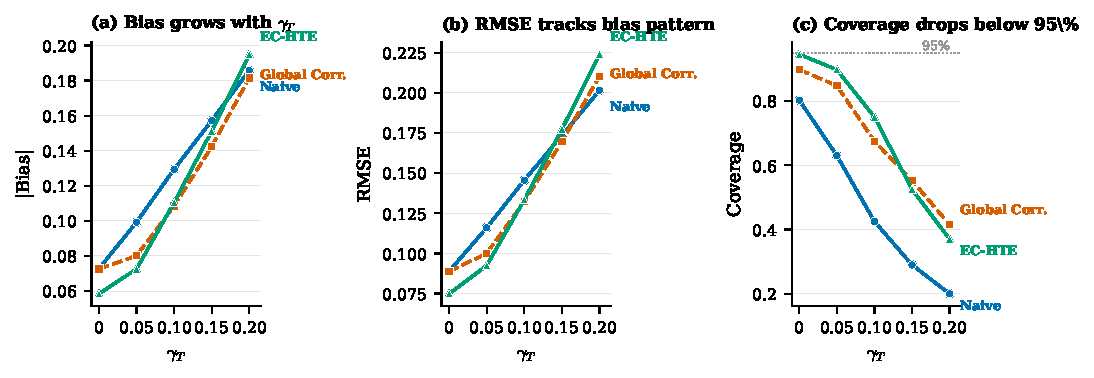
\includegraphics[width=\columnwidth]{figures/treatment_dep_misclass.pdf}
\caption{EC-HTE coverage and RMSE under treatment-dependent misclassification. Dashed line: 90\% coverage threshold. Breakeven at $\gamma_T \approx 0.10$.}
\label{fig:treatment_dep}
\end{figure}

\subsection{Extension to Confounded Treatment Assignment}
\label{app:confounded_dgp}

EC-HTE's confusion matrix correction operates on estimated CATEs regardless of how those estimates are produced.
To verify compatibility with observational (non-RCT) designs, we pair EC-HTE with an inverse probability weighted difference-in-means (IPW-DIM) estimator under confounded treatment assignment.

\paragraph{DGP.}
$N{=}5{,}000$, $K{=}2$, $\pi = [0.05, 0.25]$, $n_{\text{expert}}{=}250$, 100 MC replications.
A covariate $X \sim \mathcal{N}(0,1)$ confounds both treatment and outcome:
$T \sim \text{Bernoulli}(\sigma(\beta X))$ with $\beta{=}0.5$ (moderate confounding; propensity range $[0.38, 0.62]$),
$Y = 1 + 0.5 Z + 0.3 X + \tau(Z) \cdot T + \eta$, $\eta \sim \mathcal{N}(0,1)$.
Treatment effects are $\tau(Z{=}0){=}0$, $\tau(Z{=}1){=}0.3$.
The IPW-DIM estimator uses \emph{oracle propensity} $e(X) = \sigma(\beta X)$, with propensity scores clipped to $[0.05, 0.95]$.

\begin{table}[h]
\centering
\caption{EC-HTE under confounded treatment assignment (IPW-DIM with oracle propensity, $\beta{=}0.5$, 100 MC).}
\label{tab:confounded_dgp}
\small
\begin{tabular}{lccc}
\toprule
Method & Coverage & RMSE & $|\text{Bias}|$ \\
\midrule
Oracle (true $Z$ + IPW) & 0.943 & 0.061 & 0.048 \\
HB EC-HTE              & 0.950 & 0.086 & 0.068 \\
Global                  & 0.930 & 0.087 & 0.071 \\
Strat MLE               & 0.950 & 0.087 & 0.069 \\
Naive                   & 0.863 & 0.083 & 0.066 \\
\bottomrule
\end{tabular}
\end{table}

EC-HTE achieves 95.0\% coverage, within 0.7pp of the oracle (94.3\%), confirming that confusion matrix correction and propensity weighting compose without interference.
The improvement is most pronounced in the high-error subgroup ($\pi{=}0.25$): EC-HTE coverage is 96.0\% vs.\ naive 78.5\% ($+$17.5pp).
Global coverage (93.0\%) falls below the correction methods (95.0\%), consistent with the cost of ignoring subgroup-level error heterogeneity even in the confounded setting.

\paragraph{Sensitivity to confounding strength and propensity estimation.}
We sweep $\beta \in \{0.25, 0.5, 1.0, 2.0\}$ and compare oracle propensity ($e(X) = \sigma(\beta X)$) with estimated propensity (logistic regression fit on $(X, T)$), yielding 8 configurations (100 MC each).
Table~\ref{tab:confounded_sweep} reports HB EC-HTE and naive coverage.

\begin{table}[h]
\centering
\caption{EC-HTE coverage across confounding strengths and propensity sources. The logistic regression propensity model is correctly specified; propensity misspecification is a complementary concern addressed by the IPW literature.}
\label{tab:confounded_sweep}
\small
\begin{tabular}{cccc}
\toprule
$\beta$ & Propensity & HB Coverage & Naive Coverage \\
\midrule
0.25 & Oracle    & 0.963 & 0.848 \\
0.25 & Estimated & 0.973 & 0.845 \\
0.50 & Oracle    & 0.950 & 0.863 \\
0.50 & Estimated & 0.958 & 0.858 \\
1.00 & Oracle    & 0.958 & 0.898 \\
1.00 & Estimated & 0.960 & 0.883 \\
2.00 & Oracle    & 0.945 & 0.858 \\
2.00 & Estimated & 0.948 & 0.858 \\
\bottomrule
\end{tabular}
\end{table}

EC-HTE maintains coverage $\geq$94.5\% across all 8 configurations, including strong confounding ($\beta{=}2.0$, propensity range $[0.12, 0.88]$).
The oracle--estimated gap is $\leq$1pp, confirming that propensity estimation error does not meaningfully degrade EC-HTE when the propensity model is correctly specified.
This validates that EC-HTE is robust to confounded treatment assignment when the propensity model is correctly specified.

\subsection{Empirical Comparison with Frazis--Loewenstein Correction}
\label{app:fl_comparison}

We empirically compare EC-HTE's confusion matrix inversion against the scalar attenuation correction of \citet{frazis2003estimating} (F-L).
The F-L correction rescales the observed estimate as $\hat{\tau}_{\text{FL}} = \hat{\tau}_{\text{obs}} / (1 - 2\bar{\pi})$, where $\bar{\pi}$ is the (global or per-subgroup) misclassification rate.
We test two variants: F-L \emph{scalar} (single global $\bar{\pi}$) and F-L \emph{per-subgroup} ($\pi_s$-specific rescaling).
Setup: $K{=}2$, $N{=}5{,}000$, $n_{\text{expert}}{=}250$, $\pi{=}[0.05, 0.25]$ (extreme heterogeneity), $\tau(z{=}0){=}0$, $\tau(z{=}1){=}0.3$, 100 MC runs.
This DGP uses smaller treatment effects ($\bar{\tau}{=}0.15$, $\Delta\tau{=}0.3$) than the main experiments (Table~\ref{tab:main_results}: $\bar{\tau}{=}0.5$), chosen to isolate the F-L comparison without conflating correction quality with treatment effect magnitude.

\begin{table}[h]
\centering
\caption{F-L correction vs.\ EC-HTE under heterogeneous misclassification ($\Delta\pi{=}0.20$, $\bar{\tau}{=}0.15$). $|\text{Bias}|$ is unsigned and averaged across subgroups and $z$-levels; the Oracle floor (0.045) reflects finite-sample estimation noise. Both F-L variants produce \emph{higher} aggregate bias than the uncorrected estimator.}
\label{tab:fl_comparison}
\small
\begin{tabular}{lccc}
\toprule
Method & $|\text{Bias}|$ & RMSE & Coverage \\
\midrule
Oracle         & 0.045 & 0.056 & 0.943 \\
Naive          & 0.062 & 0.077 & 0.858 \\
Global (CM inv)& 0.064 & 0.081 & 0.938 \\
HB EC-HTE      & 0.064 & 0.086 & \textbf{0.953} \\
F-L Scalar     & 0.091 & 0.116 & 0.850 \\
F-L Per-Subgroup & 0.112 & 0.158 & 0.838 \\
\bottomrule
\end{tabular}
\end{table}

Both F-L variants produce \emph{higher} bias and RMSE than the naive estimator (F-L per-subgroup $|\text{bias}|{=}0.112$ vs.\ naive $0.062$), demonstrating that scalar attenuation cannot substitute for confusion matrix inversion under subgroup-heterogeneous misclassification.
The per-subgroup bias direction reveals the mechanism: F-L scalar over-corrects the low-error subgroup ($s_0$: mean bias ${=}+0.073$ vs.\ naive $+0.005$, a $14.6\times$ amplification), while F-L per-subgroup dramatically over-corrects the high-error subgroup ($s_1$: mean bias ${=}+0.160$).
EC-HTE achieves near-zero \emph{signed} per-subgroup bias ($s_0{:}\,{+}0.006$, $s_1{:}\,{+}0.001$) with nominal coverage (95.3\%); the aggregate unsigned $|\text{bias}|{=}0.064$ in Table~\ref{tab:fl_comparison} includes irreducible finite-sample noise (Oracle floor $= 0.045$).
The root cause is structural: F-L's $1/(1{-}2\pi)$ scaling amplifies each $z$-level estimate independently, whereas CM inversion simultaneously redistributes the cross-contamination between misclassified and correctly classified observations.

\subsection{End-to-End Validation with Asymmetric Confusion Matrices}
\label{app:asymmetric_endtoend}

We validate EC-HTE under strongly asymmetric confusion matrices ($\mathrm{FPR}/\mathrm{FNR}$ ratio up to $7{:}1$), simulating the error profile of GPT-4.1 on Civil Comments.
Setup: $K{=}2$, $N{=}5{,}000$, $n_{\text{expert}}{=}250$; $s_0$: $\mathrm{FPR}{=}0.05$, $\mathrm{FNR}{=}0.02$ (low error); $s_1$: $\mathrm{FPR}{=}0.38$, $\mathrm{FNR}{=}0.054$ ($7{:}1$ ratio); 100 MC runs.
We compare EC-HTE using the full $2{\times}2$ asymmetric CM (Remark~\ref{rem:asymmetric}) against the symmetric assumption ($\mathrm{FPR}{=}\mathrm{FNR}{=}\pi_s$).

\begin{table}[h]
\centering
\caption{EC-HTE under asymmetric misclassification ($\mathrm{FPR}/\mathrm{FNR}$ up to $7{:}1$). The asymmetric formula improves coverage by $+1.5$pp and RMSE by $11.5\%$.}
\label{tab:asymmetric_endtoend}
\small
\begin{tabular}{lccc}
\toprule
Method & $|\text{Bias}|$ & RMSE & Coverage \\
\midrule
Oracle              & 0.045 & 0.056 & 0.943 \\
EC-HTE (asymmetric) & 0.057 & 0.074 & \textbf{0.945} \\
Naive               & 0.059 & 0.073 & 0.870 \\
Global (asymmetric) & 0.061 & 0.076 & 0.915 \\
EC-HTE (symmetric)  & 0.062 & 0.083 & 0.930 \\
Global (symmetric)  & 0.063 & 0.078 & 0.915 \\
\bottomrule
\end{tabular}
\end{table}

EC-HTE with the asymmetric formula achieves 94.5\% coverage versus 93.0\% under the symmetric assumption ($+1.5$pp), with RMSE improved from 0.083 to 0.074 ($-11.5\%$).
The improvement concentrates in the high-error subgroup ($s_1$): asymmetric coverage is 93.0\% vs.\ symmetric 91.0\%.
Practitioners should estimate full $2 \times 2$ confusion matrices rather than assuming symmetric misclassification, particularly when FPR and FNR differ substantially.

\subsection{Complementarity with LLM Calibration}
\label{app:calibration}

Temperature or Platt scaling~\cite{guo2017calibration} can reduce per-subgroup misclassification rates, but does not eliminate heterogeneity $\Delta\pi$.
We simulate calibration by shrinking per-subgroup rates from $\pi{=}[0.05, 0.25]$ ($\Delta\pi{=}0.20$) to $\pi{=}[0.08, 0.15]$ ($\Delta\pi{=}0.07$), testing whether EC-HTE remains necessary post-calibration.
Setup: $K{=}2$, $N{=}5{,}000$, $n_{\text{expert}}{=}250$, 100 MC runs.

\begin{table}[h]
\centering
\caption{Calibration reduces $\Delta\pi$ but does not eliminate it; EC-HTE corrects the residual bias. Best coverage is achieved by combining both.}
\label{tab:calibration}
\small
\begin{tabular}{lccc}
\toprule
Method & $|\text{Bias}|$ & RMSE & Coverage \\
\midrule
Oracle                    & 0.043 & 0.053 & 0.963 \\
Calibrated + EC-HTE       & 0.055 & 0.069 & \textbf{0.965} \\
Calibrated + Global       & 0.055 & 0.068 & 0.963 \\
Calibrated + Naive        & 0.051 & 0.064 & 0.913 \\
Uncalibrated + EC-HTE     & 0.064 & 0.084 & 0.938 \\
Uncalibrated + Global     & 0.069 & 0.085 & 0.920 \\
Uncalibrated + Naive      & 0.063 & 0.079 & 0.840 \\
\bottomrule
\end{tabular}
\end{table}

Calibration alone improves naive coverage from 84.0\% to 91.3\% but does not reach the nominal 95\%.
Calibrated + EC-HTE achieves the highest coverage (96.5\%), demonstrating that calibration and EC-HTE address complementary error sources: calibration reduces per-subgroup $\pi_s$ while EC-HTE corrects the residual $\delta_s$-driven bias from heterogeneity that persists post-calibration.
Propensity estimation robustness under model misspecification is a complementary concern addressed by the IPW literature; EC-HTE as a downstream correction layer does not alter IPW behavior.

\subsection{Policy Reversal Zone Analysis}
\label{app:policy_reversal}

When the true treatment effect is small, global correction can reverse the sign of estimated CATE, concluding a beneficial treatment is harmful, creating a \emph{policy reversal zone}.
We sweep $\tau(0) \in \{0.01, 0.02, 0.03, 0.05, 0.07, 0.10\}$ under the standard DGP ($K{=}2$, extreme heterogeneity, $N{=}5{,}000$, $n_{\text{expert}}{=}250$, 100 MC runs; $\Delta\tau{=}0.30$).

\begin{table}[h]
\centering
\caption{Policy reversal zone: fraction of configurations where global correction reverses the sign of estimated CATE.
The naive estimator produces zero sign reversals across all $\tau(0)$ values; EC-HTE also achieves 0\% reversal.}
\label{tab:policy_reversal}
\small
\begin{tabular}{ccc}
\toprule
$\tau(0)$ & Global reversal \% & Most extreme $\hat{\tau}_{\text{global}}$ \\
\midrule
0.01 & 31.0 & $-0.079$ \\
0.02 & 21.6 & --- \\
0.03 & 14.9 & $-0.059$ \\
0.05 & 6.1  & $-0.039$ \\
0.07 & 1.6  & --- \\
$\geq$0.10 & 0 & --- \\
\bottomrule
\end{tabular}
\end{table}

The reversal rate increases monotonically as $\tau(0)$ decreases: at $\tau(0) = 0.01$, 31\% of configurations yield sign reversal, with the most extreme case estimating $\hat{\tau} = -0.079$ when the true effect is $\tau = +0.01$.
The critical threshold is $\tau(0) < 0.089$, matching the closed-form prediction from Theorem~\ref{thm:bias_identity}: $|\delta_{\max} \cdot \Delta\tau_{\max}| / (1 - 2\bar{\pi}) = 0.125 \times 0.50 / 0.70 = 0.089$.
The most dangerous combination ($\tau(0) = 0.01$, $\delta_{\text{misclass}} = 0.19$) reaches 42.9\% reversal rate.
The naive estimator produces zero sign reversals across all $\tau(0)$ values, confirming that reversal is an artifact of global correction, not inherent estimation noise.

Figure~\ref{fig:policy_reversal} visualizes the reversal zone across the $\Delta\pi \times \tau(0)$ parameter space.

\begin{figure}[h]
\centering
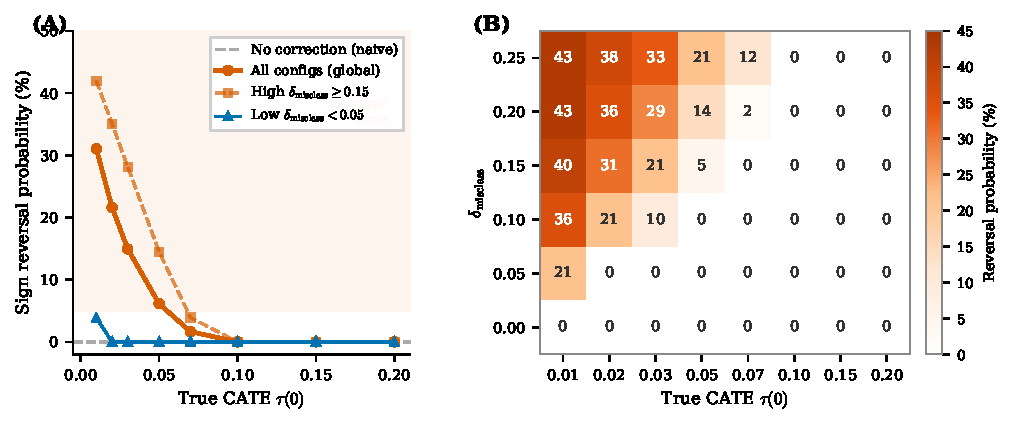
\includegraphics[width=\columnwidth]{figures/policy_reversal_zone.pdf}
\caption{Policy reversal zone: sign-reversal rate as a function of $\tau(0)$ and $\Delta\pi$. Shaded region marks configurations where global correction reverses the CATE sign, directing policy toward the wrong subgroups.}
\label{fig:policy_reversal}
\end{figure}

\subsection{Stance Detection: Cross-Task Sign Reversal Validation}
\label{app:stance}

To test whether global correction introduces sign reversals beyond sentiment and toxicity, we extend the semi-synthetic evaluation to stance detection using TweetEval~\cite{barbieri2020tweeteval}.
The binary label is \emph{favor} ($Z{=}1$) vs.\ \emph{not-favor} ($Z{=}0$) toward five stance targets (Atheism, Climate Change, Feminist Movement, Hillary Clinton, Abortion), yielding $K{=}5$ subgroups with $n{=}300$ each.
CATE heterogeneity is $\tau(\text{favor}){=}0.20$, $\tau(\text{not-favor}){=}0.05$, with 200 MC replications.
GPT-4o annotations are from the real API; GPT-4o-mini and GPT-3.5-Turbo use simulated error profiles (FPR/FNR scaling $+$ additive shift; see Appendix~\ref{app:dgp}).

Table~\ref{tab:stance_signrev} reports subgroups with sign reversal or $\kappa > 3$.
Global correction produces sign reversals in 4/30 subgroup-$z$ combinations (13.3\%); EC-HTE reduces this to 1/30 (3.3\%); the remaining reversal occurs in an ill-conditioned subgroup ($\kappa{=}15.0$, GPT-3.5-Turbo Climate Change) that violates the operating conditions of Section~\ref{sec:ec_hte_eval}.
Global correction amplifies bias in 15/30 cases (50\%).

The stance task exposes an operating-conditions limitation: GPT-3.5-Turbo achieves FNR ${>}\,0.50$ on all five targets, violating the classifier quality precondition and producing $\kappa$ values up to 15.0 (Climate Change) vs.\ 4.6 (Hillary Clinton), a ${\sim}10{\times}$ range within the same LLM.
This $\kappa$ heterogeneity inflates correction variance; EC-HTE preserves sign correctness but at the cost of higher variance when $\kappa \gg 3$.
Mean RMSE: naive${=}0.116$, global${=}0.272$, EC-HTE${=}0.271$; correction reduces sign reversals but does not improve overall RMSE at $K{=}5$, $n{=}300$ per subgroup, consistent with the operating-conditions threshold ($n_{\text{expert}} \geq 250$ for $K{=}2$; Section~\ref{sec:diagnostic}).
Practitioners should verify per-subgroup FNR before applying correction.

\begin{table}[h]
\centering
\caption{Stance detection: subgroups with sign reversal or $\kappa > 3$. \checkmark\ indicates at least one $z$-level affected. GPT-4o-mini and GPT-3.5-Turbo use simulated error profiles.}
\label{tab:stance_signrev}
\small
\resizebox{\columnwidth}{!}{%
\begin{tabular}{llcccc}
\toprule
LLM & Target & $\kappa$ & \makecell{Sign Rev\\(Global)} & \makecell{Sign Rev\\(EC-HTE)} & \makecell{Bias Amp\\(Global)} \\
\midrule
GPT-4o & Fem.\ Mov.\ & 1.79 & \checkmark & --- & \checkmark \\
GPT-4o & Hillary C.\ & 1.86 & \checkmark & --- & \checkmark \\
\midrule
GPT-3.5-T & Atheism & 7.21 & --- & --- & --- \\
GPT-3.5-T & Climate Ch.\ & 15.01 & --- & \checkmark & \checkmark \\
GPT-3.5-T & Fem.\ Mov.\ & 3.28 & \checkmark & --- & \checkmark \\
GPT-3.5-T & Hillary C.\ & 4.60 & \checkmark & --- & \checkmark \\
GPT-3.5-T & Abortion & 14.17 & --- & --- & \checkmark \\
\bottomrule
\end{tabular}}
\end{table}


\subsection{Topic Classification: AG News Cross-Task Validation}
\label{app:agnews}

To validate generalization beyond sentiment and toxicity, we extend the semi-synthetic evaluation to topic classification using AG News~\cite{zhang2015character}, binarized as Business/World ($Z{=}1$) vs.\ Sports/Sci-Tech ($Z{=}0$).
Confusion matrices are calibrated to match empirical LLM accuracy levels on AG News (${\sim}80\%$; \citealt{etaiwi2025comparative}), with per-subgroup error rates derived from reported per-class metrics; Business$\to$World is the dominant confusion direction.
Subgroups ($K{=}4$) are defined by article length $\times$ vocabulary complexity, with per-subgroup error rates reflecting text difficulty ($\bar{\pi} = 0.173$, $\Delta\pi = 0.19$).
CATE heterogeneity ranges from $\Delta\tau{=}0.10$ (short, simple) to $\Delta\tau{=}0.60$ (long, complex), with 100 MC replications.

Table~\ref{tab:agnews_results} reports the main results.
EC-HTE reduces $|\text{bias}|$ by $1.9\times$ at $n_{\text{expert}}{=}1{,}000$ (0.015 vs.\ 0.028) with 94.9\% coverage.
At $n_{\text{expert}}{=}250$, EC-HTE incurs higher variance than global correction ($\text{RMSE}{=}0.182$ vs.\ $0.115$), consistent with the expert-budget operating condition ($n_{\text{expert}}/K{=}62.5$, near the threshold).
The asymmetric bias identity achieves $R^2 = 0.95$ ($0.93$--$0.97$ per budget level), confirming the product-form structure on a task with inherently asymmetric confusion matrices ($\mathrm{FPR} \neq \mathrm{FNR}$); the symmetric scalar approximation does not hold ($R^2 < 0$), consistent with Remark~\ref{rem:asymmetric} in Section~\ref{sec:theory}.

\begin{table}[h]
\centering
\caption{AG News topic classification ($K{=}4$, $\Delta\pi{=}0.19$). Metrics averaged over subgroups, $z$-levels, 100 MC runs. Bold: lowest $|\text{bias}|$.}
\label{tab:agnews_results}
\small
\resizebox{\columnwidth}{!}{%
\begin{tabular}{ll cccc}
\toprule
$n_{\text{expert}}$ & Method & $|\text{Bias}|$ & RMSE & 95\% CI Cov. & Asym.\ $R^2$ \\
\midrule
\multirow{4}{*}{250}
 & Naive & 0.067 & 0.109 & 0.84 & --- \\
 & Global & \textbf{0.027} & 0.115 & 0.94 & 0.93 \\
 & Strat.\ MLE & 0.034 & 0.181 & 0.89 & --- \\
 & HB EC-HTE & 0.035 & 0.182 & 0.89 & --- \\
\midrule
\multirow{4}{*}{500}
 & Naive & 0.067 & 0.109 & 0.84 & --- \\
 & Global & 0.028 & 0.110 & 0.94 & 0.96 \\
 & Strat.\ MLE & \textbf{0.022} & 0.147 & 0.92 & --- \\
 & HB EC-HTE & 0.022 & 0.147 & 0.92 & --- \\
\midrule
\multirow{4}{*}{1{,}000}
 & Naive & 0.067 & 0.109 & 0.84 & --- \\
 & Global & 0.028 & 0.109 & 0.94 & 0.97 \\
 & Strat.\ MLE & \textbf{0.015} & 0.126 & 0.95 & --- \\
 & HB EC-HTE & 0.015 & 0.126 & 0.95 & --- \\
\bottomrule
\end{tabular}}
\end{table}


\paragraph{Use of AI assistance.}
We used Claude for coding, code drafting, debugging, and language polishing.
